\documentclass[12pt,a4paper]{article}
\usepackage[utf8]{inputenc}\usepackage[T1]{fontenc}\usepackage[brazil]{babel}\usepackage{lmodern}
\usepackage{geometry}\geometry{margin=2.3cm}\usepackage{graphicx}\graphicspath{{figuras/}}
\usepackage{booktabs,tabularx,array,amsmath,amssymb,siunitx,xcolor,float}\sisetup{output-decimal-marker={,}}
\usepackage[section]{placeins}\usepackage{enumitem,microtype,caption,subcaption,listings,hyperref,fancyhdr}
\hypersetup{colorlinks=true,linkcolor=blue!55!black,urlcolor=blue!55!black,citecolor=blue!55!black}
\lstdefinestyle{sindyeq}{basicstyle=\ttfamily\scriptsize,breaklines=true,breakatwhitespace=false,columns=fullflexible,frame=single,numbers=left,numberstyle=\tiny\color{gray},xleftmargin=1.5em,framexleftmargin=1.2em,showstringspaces=false}
\pagestyle{fancy}\fancyhf{}\lhead{Dam-break laminar e modelos reduzidos}\rhead{Relatório técnico}\cfoot{\thepage}
\setlength{\parindent}{1.2em}\setlength{\parskip}{0.35em}\newcommand{\code}[1]{\texttt{#1}}
\title{\textbf{Relatório técnico do caso dam-break laminar}\\[0.4em]OpenFOAM, POD, SAE e identificação dinâmica SINDy}
\author{Análise dos códigos e resultados armazenados no caso}\date{\today}
\begin{document}\maketitle
\begin{abstract}
Este relatório documenta o caso dam-break laminar calculado com OpenFOAM 13, sua redução por POD e SAE e a identificação dinâmica por POD--SINDy, SAE--SINDy e SAE--POD--SINDy. A POD multivariável com 50 modos preserva 99,62\% da energia e apresenta erro global de 6,17\%; entretanto, inclui um canal $k$ artificialmente nulo. O SAE comprime cinco canais físicos em oito latentes, mas apresenta forte perda de generalização temporal ($R^2_{val}=0,133$). POD--SINDy e SAE--SINDy falham em integração livre. A POD estabilizadora reduz oito latentes para quatro, conserva 90,95\% da energia e permite integração livre, com erro relativo 0,634 e $R^2=0,598$. O comportamento é relacionado ao papel estabilizador proposto por Lin, Xiao e Fang, sem confundir reconstrução de snapshots com captura da dinâmica.
\end{abstract}
\tableofcontents\listoffigures\listoftables\clearpage

\section{Escopo e ressalvas de proveniência}
O caso está em
\begin{quote}\small\path{/home/mlep-pc-ubuntu/OpenFOAM/mlep-pc-ubuntu-13/run/damBreakLaminar 10 000}.\end{quote}
Foram examinados dicionários OpenFOAM, notebooks, modelos Keras e resultados NPZ/JSON/CSV. Não houve reexecução.

A POD solicita $U$, $\alpha_{water}$, $p_{rgh}$ e $k$. Como uma simulação laminar não grava $k$, a rotina captura o erro de leitura e insere zeros. Portanto, a dimensão declarada é 11340 ($5\times2268$), mas um quinto dela é canal nulo. Já o SAE usa $U_x,U_y,\alpha_{water},p_{rgh},\rho$, com $\rho=\alpha\rho_{water}+(1-\alpha)\rho_{air}$. Assim, POD e SAE não reduzem exatamente o mesmo estado físico.

\section{Modelo de alta fidelidade OpenFOAM}
\subsection{Física, geometria e malha}
O solver \code{incompressibleVoF} simula água e ar com tensão superficial \SI{0.07}{N.m^{-1}} e gravidade $(0,-9{,}81,0)\,\si{m.s^{-2}}$. A coluna inicial de água ocupa $0\le x\le\SI{0.1461}{m}$ e $0\le y\le\SI{0.292}{m}$. A água tem $\rho=1000\,\si{kg.m^{-3}}$, $\nu=10^{-6}\,\si{m^2.s^{-1}}$; o ar, $\rho=1\,\si{kg.m^{-3}}$, $\nu=1{,}48\times10^{-5}\,\si{m^2.s^{-1}}$.

O domínio nominal é $0{,}584\times0{,}584\times0{,}0146\,\si{m^3}$, dividido em cinco blocos e 2268 células. Há uma célula em $z$ e patches padrão \code{empty}, caracterizando aproximação bidimensional. Esquerda, direita e fundo são paredes; o topo é atmosfera. O arquivo \code{momentumTransport} define explicitamente \code{simulationType laminar}.

\subsection{Discretização e solvers}
\begin{table}[H]\centering\caption{Parâmetros numéricos OpenFOAM.}\label{tab:foam}
\begin{tabularx}{\textwidth}{>{\bfseries}l X}\toprule Item&Configuração\\\midrule
Tempo&Euler de primeira ordem; $\Delta t=10^{-4}\,\si{s}$ fixo; $0\le t\le1\,\si{s}$\\
Saída&todo passo: 10001 snapshots\\
Gradiente&Gauss linear\\
Convecção VOF&\code{interfaceCompression vanLeer 1}\\
Convecção de momento&Gauss \code{linearUpwind grad(U)}\\
Difusão&Gauss linear uncorrected\\
Interpolação/$\mathrm{snGrad}$&linear / uncorrected\\
Passo adaptativo&desativado; limites de Courant não controlam $\Delta t$\\
\bottomrule\end{tabularx}\end{table}

\begin{table}[H]\centering\caption{Solução algébrica e acoplamento.}\label{tab:solvers}
\begin{tabularx}{\textwidth}{>{\bfseries}l X}\toprule Bloco&Configuração\\\midrule
$\alpha_{water}$&2 corretores, 1 subciclo; MULES 10 iterações; tolerância linear $10^{-8}$\\
$p_{rgh}$&PCG/DIC; tolerância $10^{-7}$; \code{relTol}=0,05 e zero no final\\
$U$&\code{smoothSolver}/\code{symGaussSeidel}; tolerância $10^{-6}$\\
PIMPLE&1 corretor externo, 3 internos, nenhum não ortogonal; preditor desligado\\
\bottomrule\end{tabularx}\end{table}

São positivos o passo pequeno e a elevada resolução de saída. São limitações o esquema temporal de primeira ordem, ausência de controle adaptativo de Courant, uma célula em $z$ e ausência de estudos de malha, passo ou validação experimental.

\section{POD multivariável}
A matriz centralizada e normalizada por snapshot é decomposta por
\begin{equation}X-\overline X=U\Sigma V^T,\qquad X_r=U_r\Sigma_rV_r^T.\end{equation}
Foram usados 10001 snapshots, 2268 células, cinco canais declarados e até 50 modos.

\begin{table}[H]\centering\caption{Energia e erro POD.}\label{tab:pod}
\begin{tabular}{rcc}\toprule Modos&Energia acumulada&Erro global\\\midrule
1&0,3975&0,7762\\2&0,5632&0,6609\\4&0,7727&0,4767\\8&0,8772&0,3505\\16&0,9494&0,2249\\32&0,9870&0,1140\\50&0,9962&0,0617\\\bottomrule\end{tabular}\end{table}

\begin{figure}[H]\centering
\begin{subfigure}{.49\textwidth}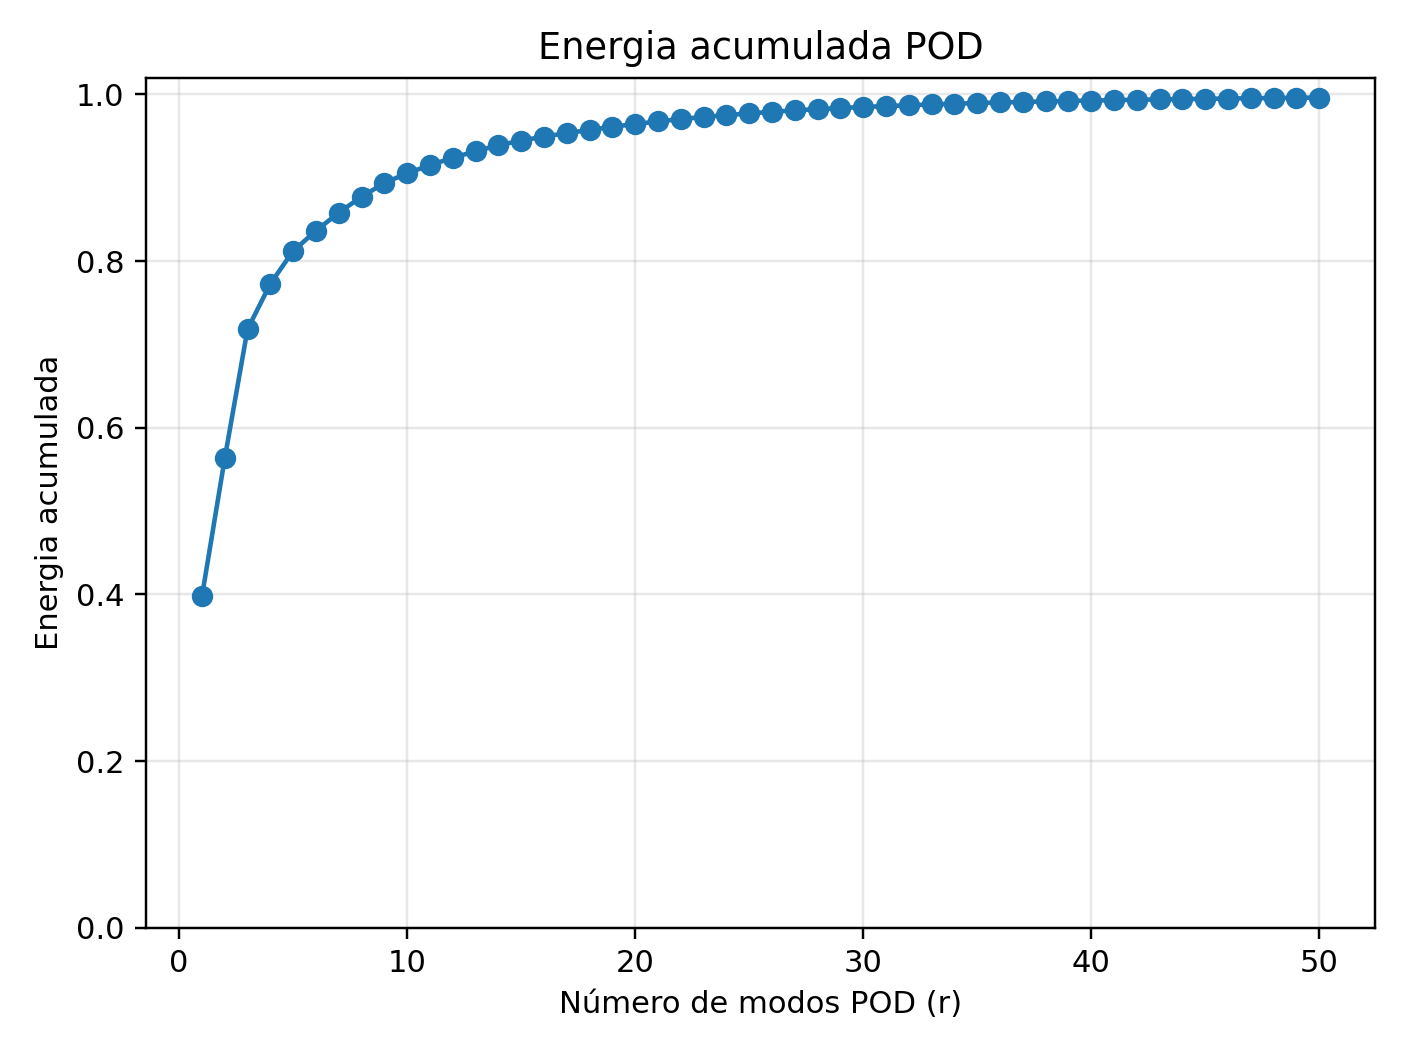
\includegraphics[width=\linewidth]{pod_energia.png}\caption{Energia.}\end{subfigure}
\begin{subfigure}{.49\textwidth}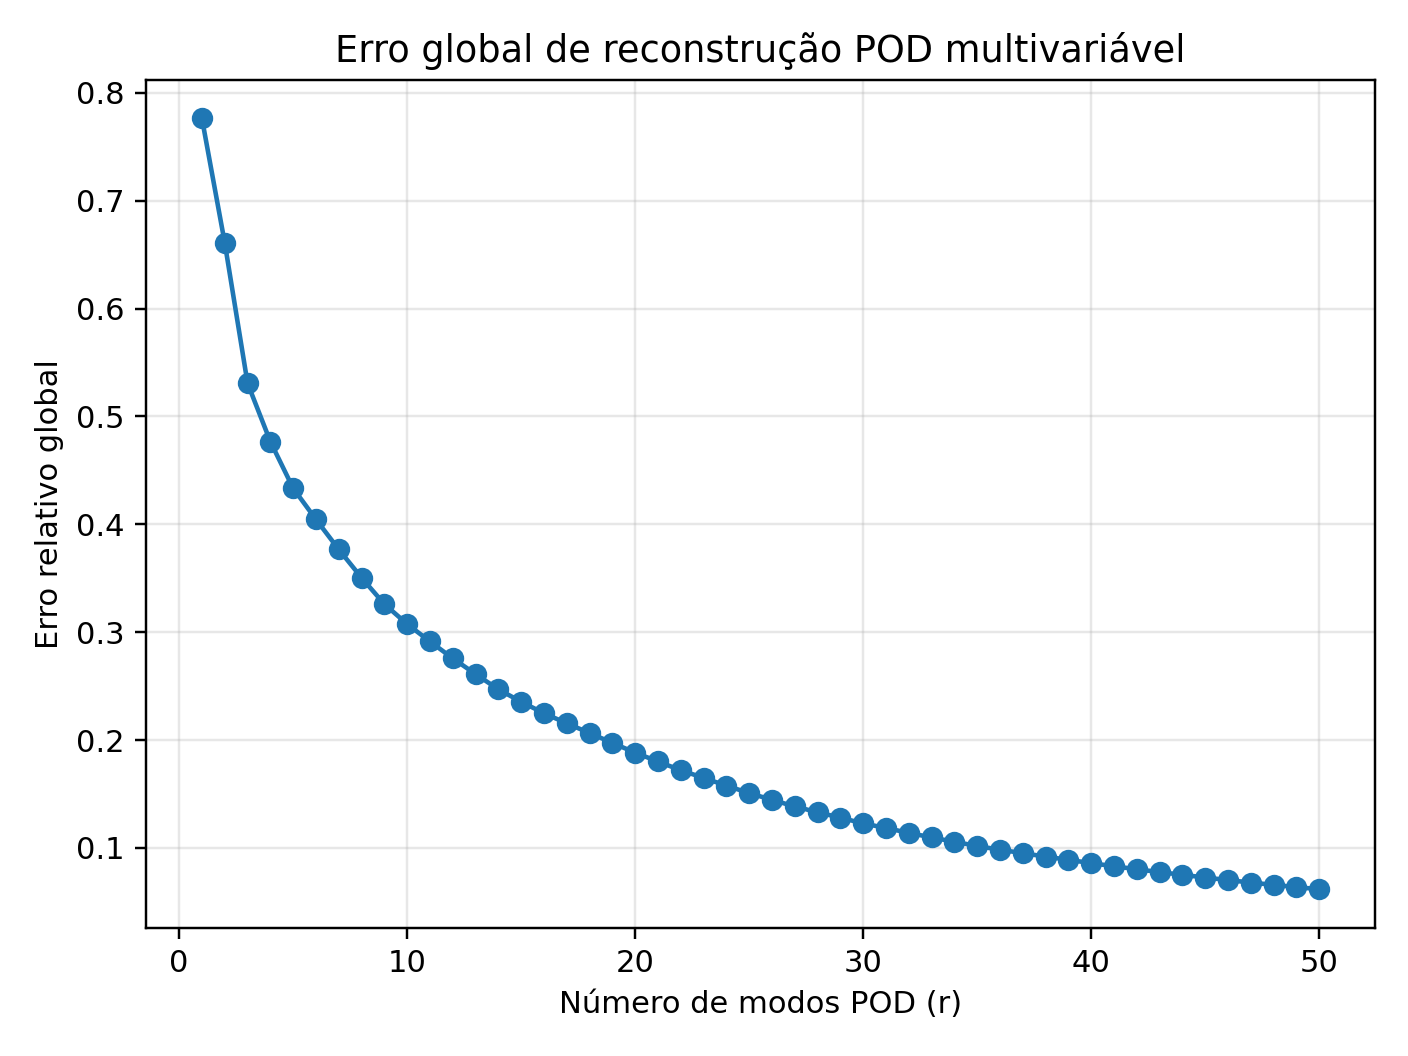
\includegraphics[width=\linewidth]{pod_erro.png}\caption{Erro.}\end{subfigure}
\caption{Convergência POD.}\end{figure}
\begin{figure}[H]\centering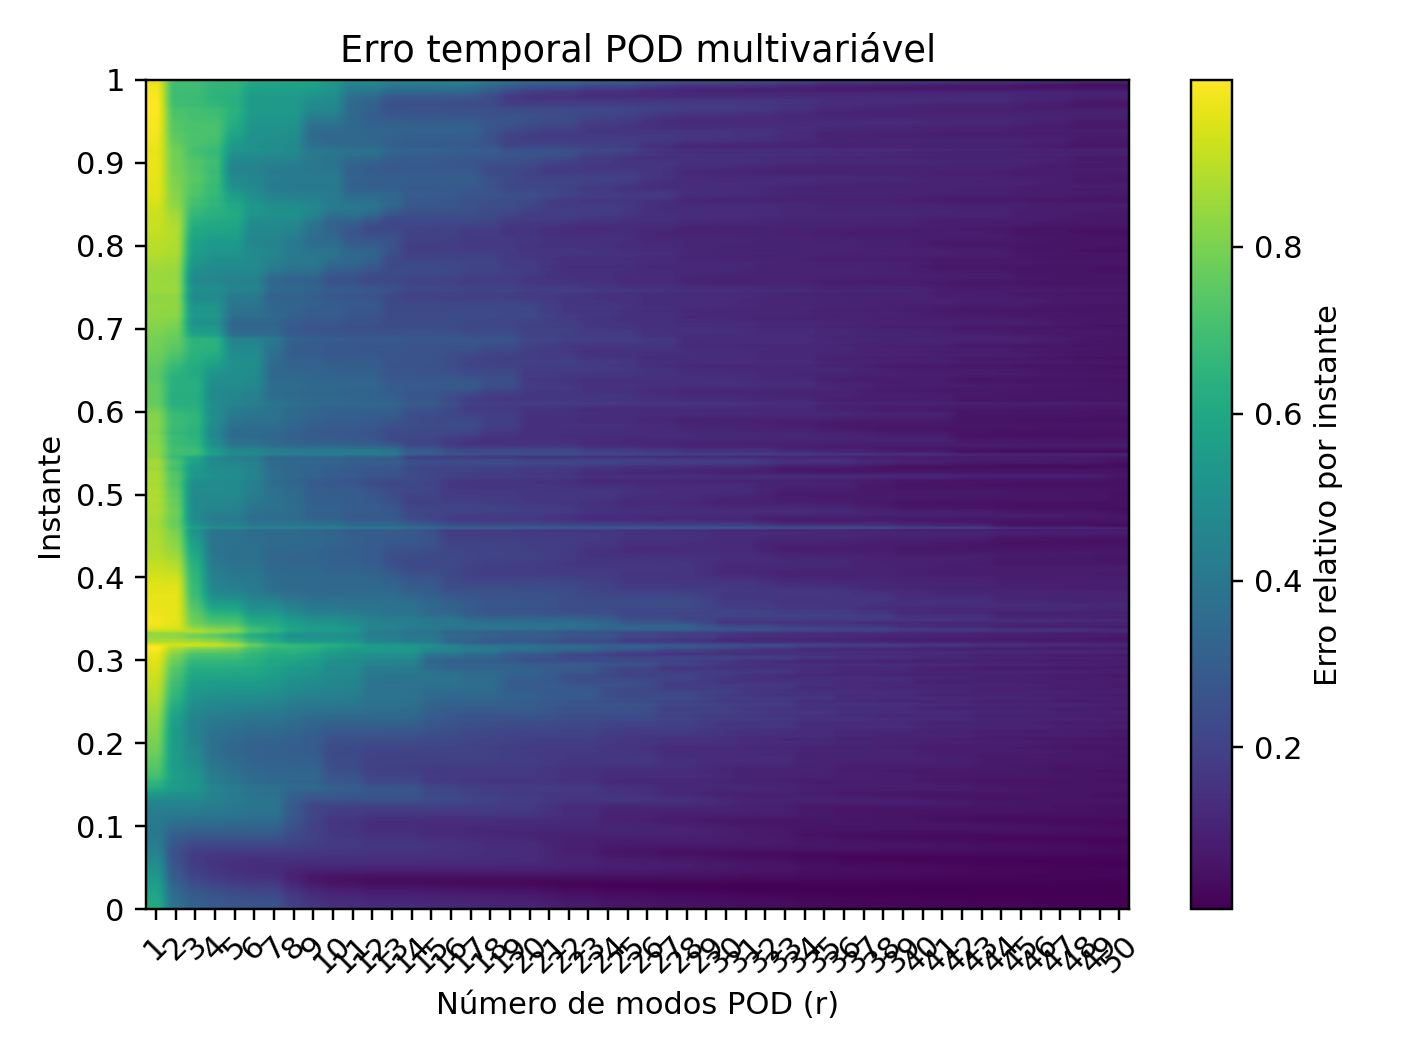
\includegraphics[width=.9\textwidth]{pod_mapa.png}\caption{Mapa temporal do erro POD. O erro máximo com 50 modos é 0,837, concentrado no fim do intervalo.}\end{figure}
\begin{figure}[H]\centering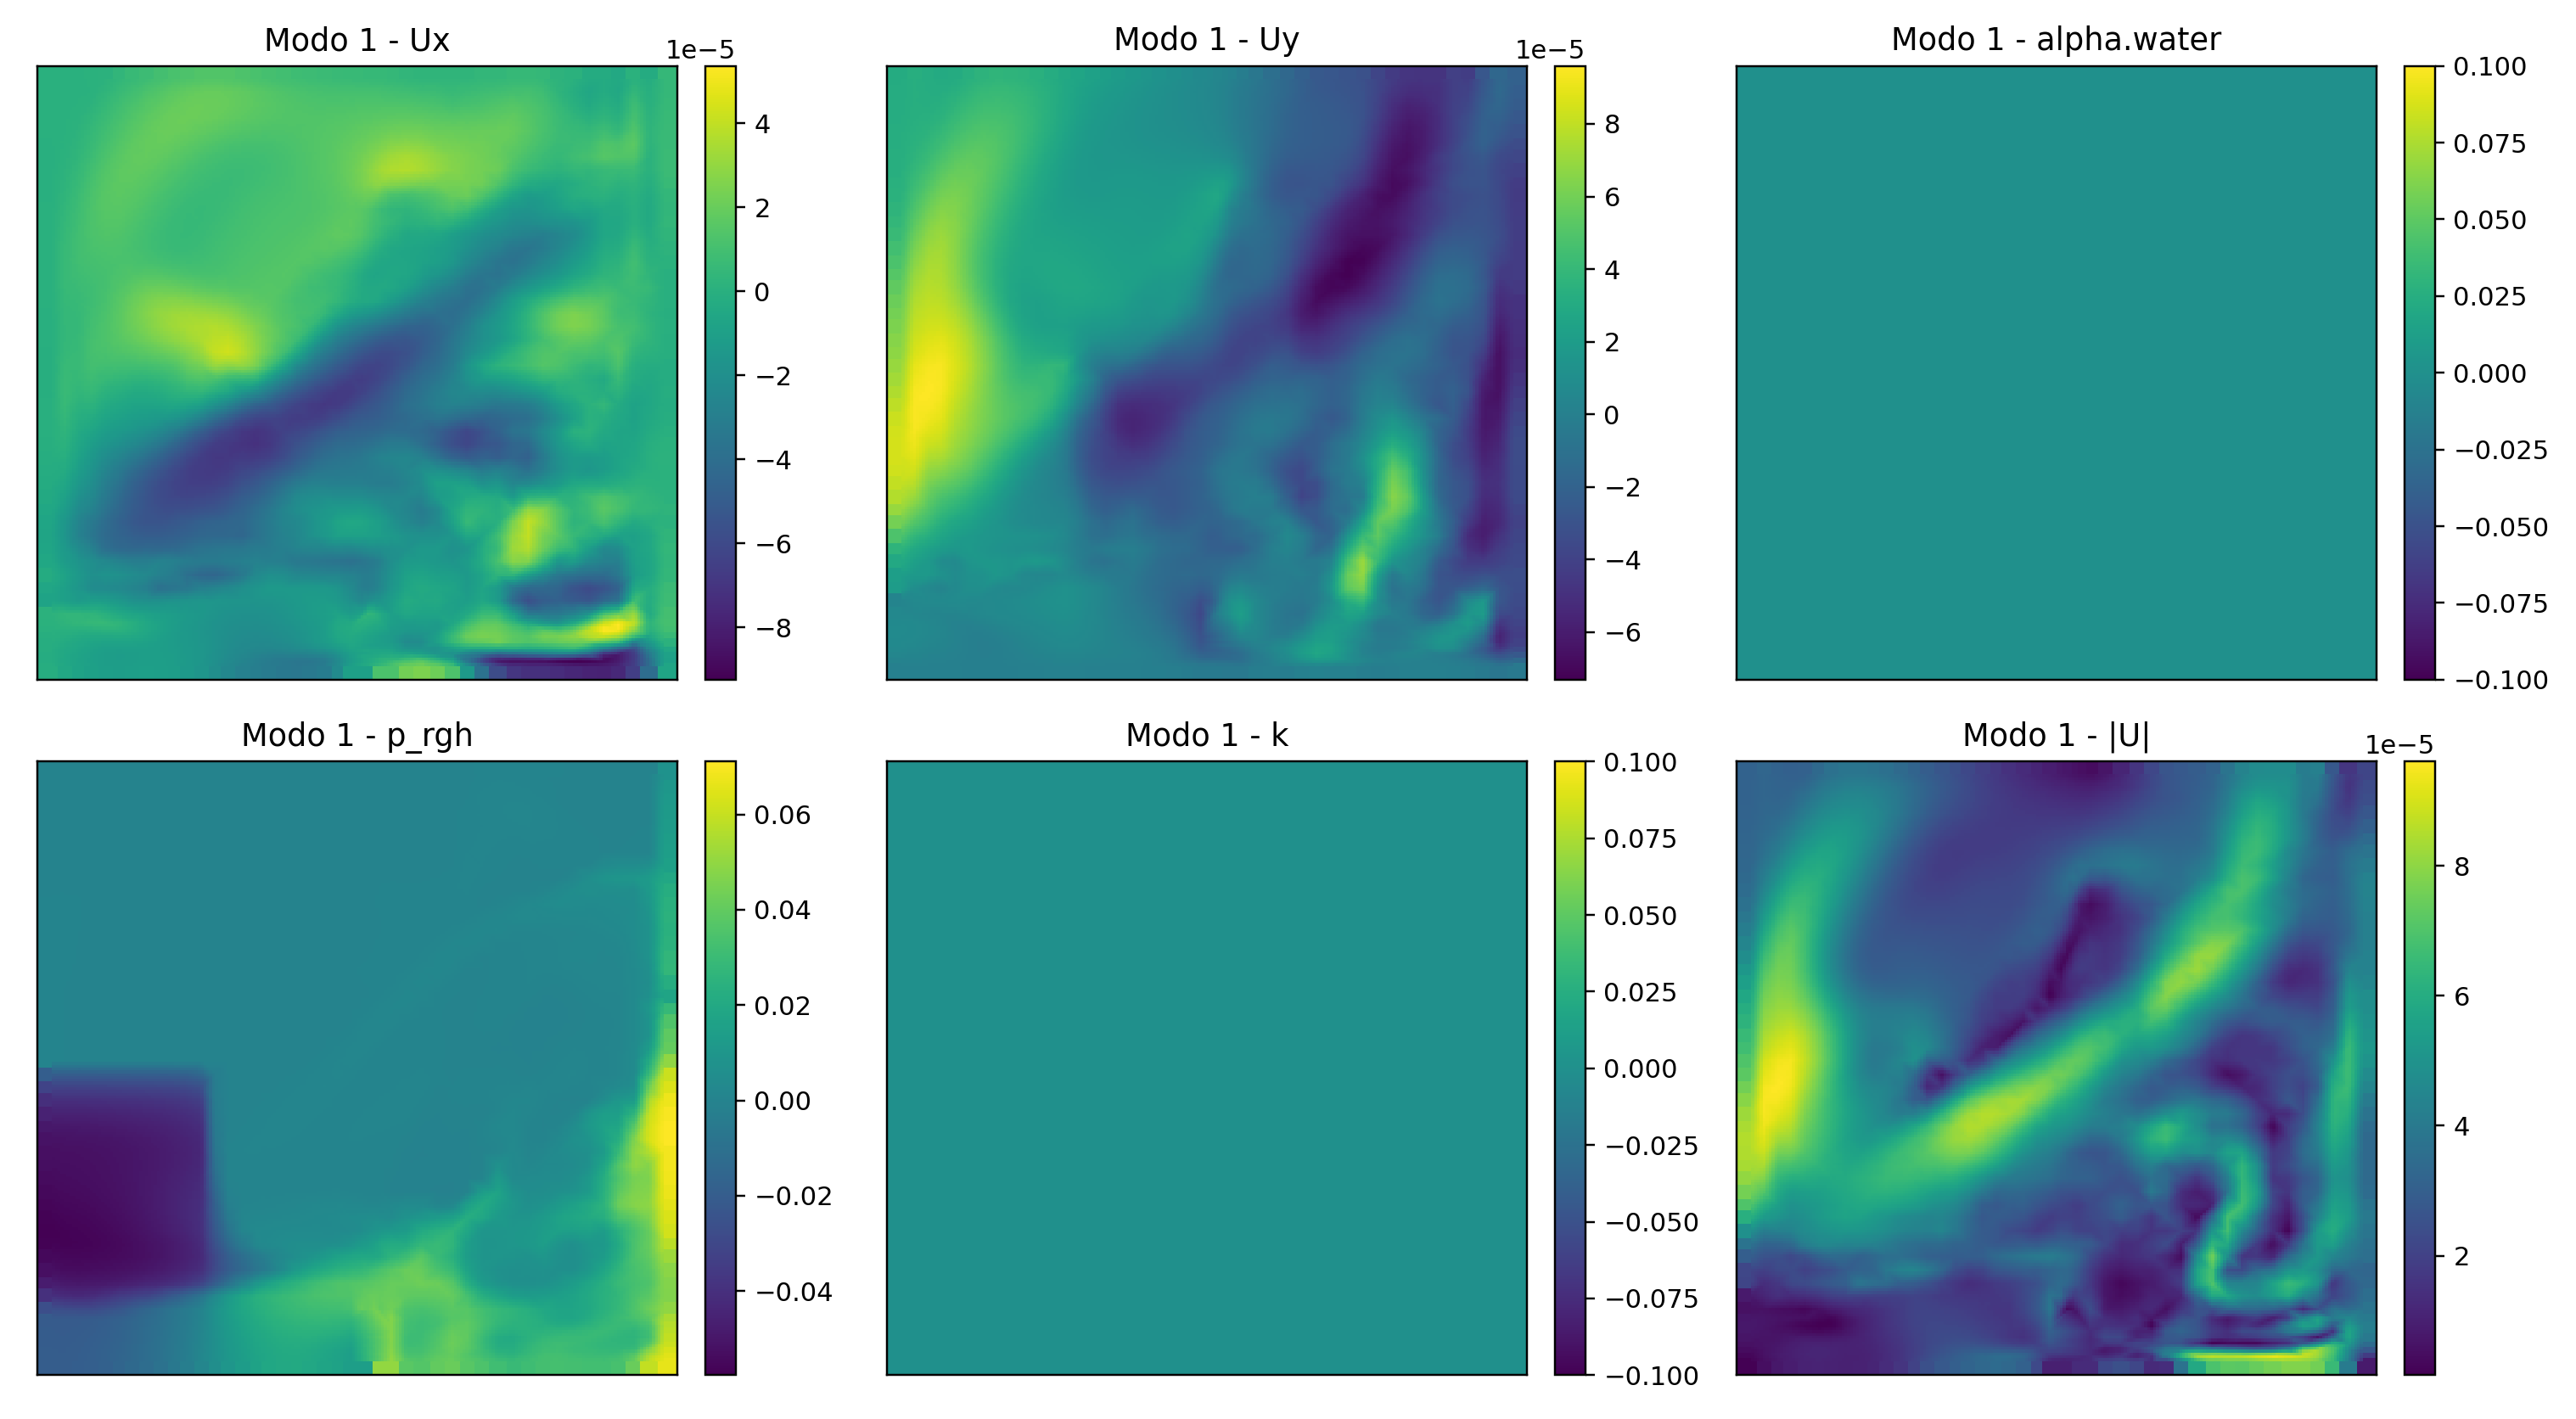
\includegraphics[width=.95\textwidth]{pod_modo1.png}\caption{Primeiro modo POD em todos os canais; $k$ é nulo por construção.}\end{figure}
\begin{figure}[H]\centering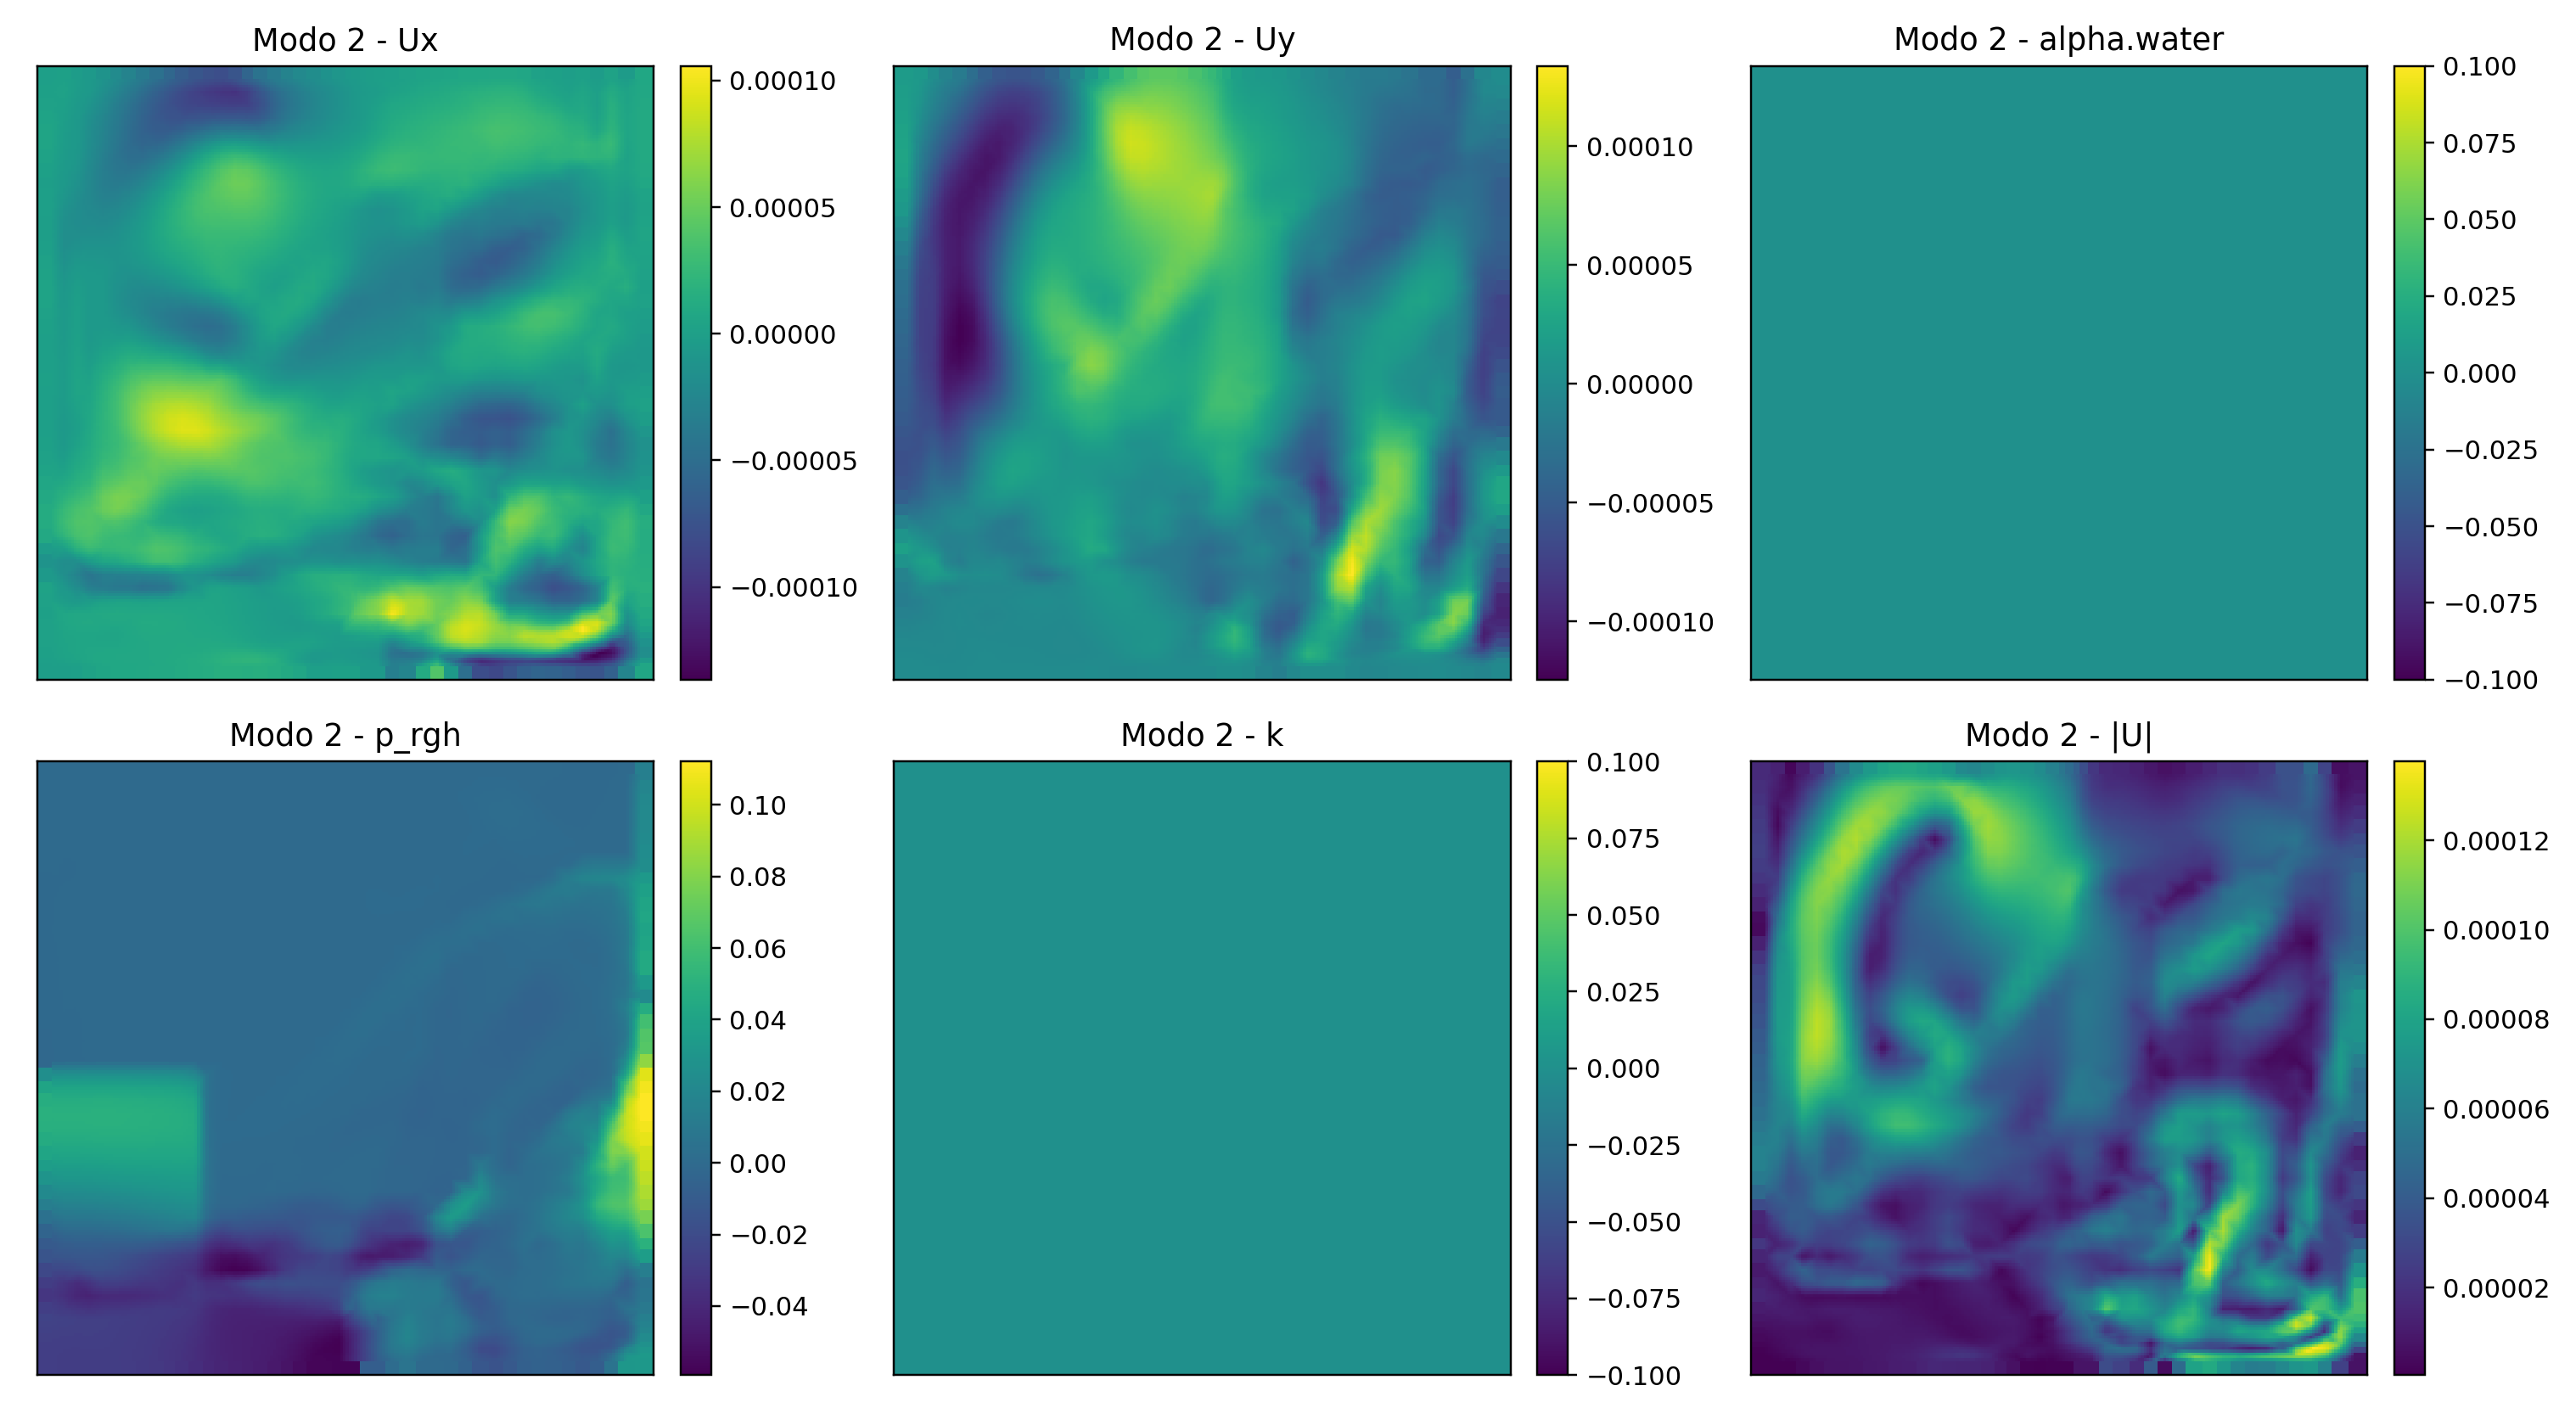
\includegraphics[width=.95\textwidth]{pod_modo2.png}\caption{Segundo modo POD.}\end{figure}
\begin{figure}[H]\centering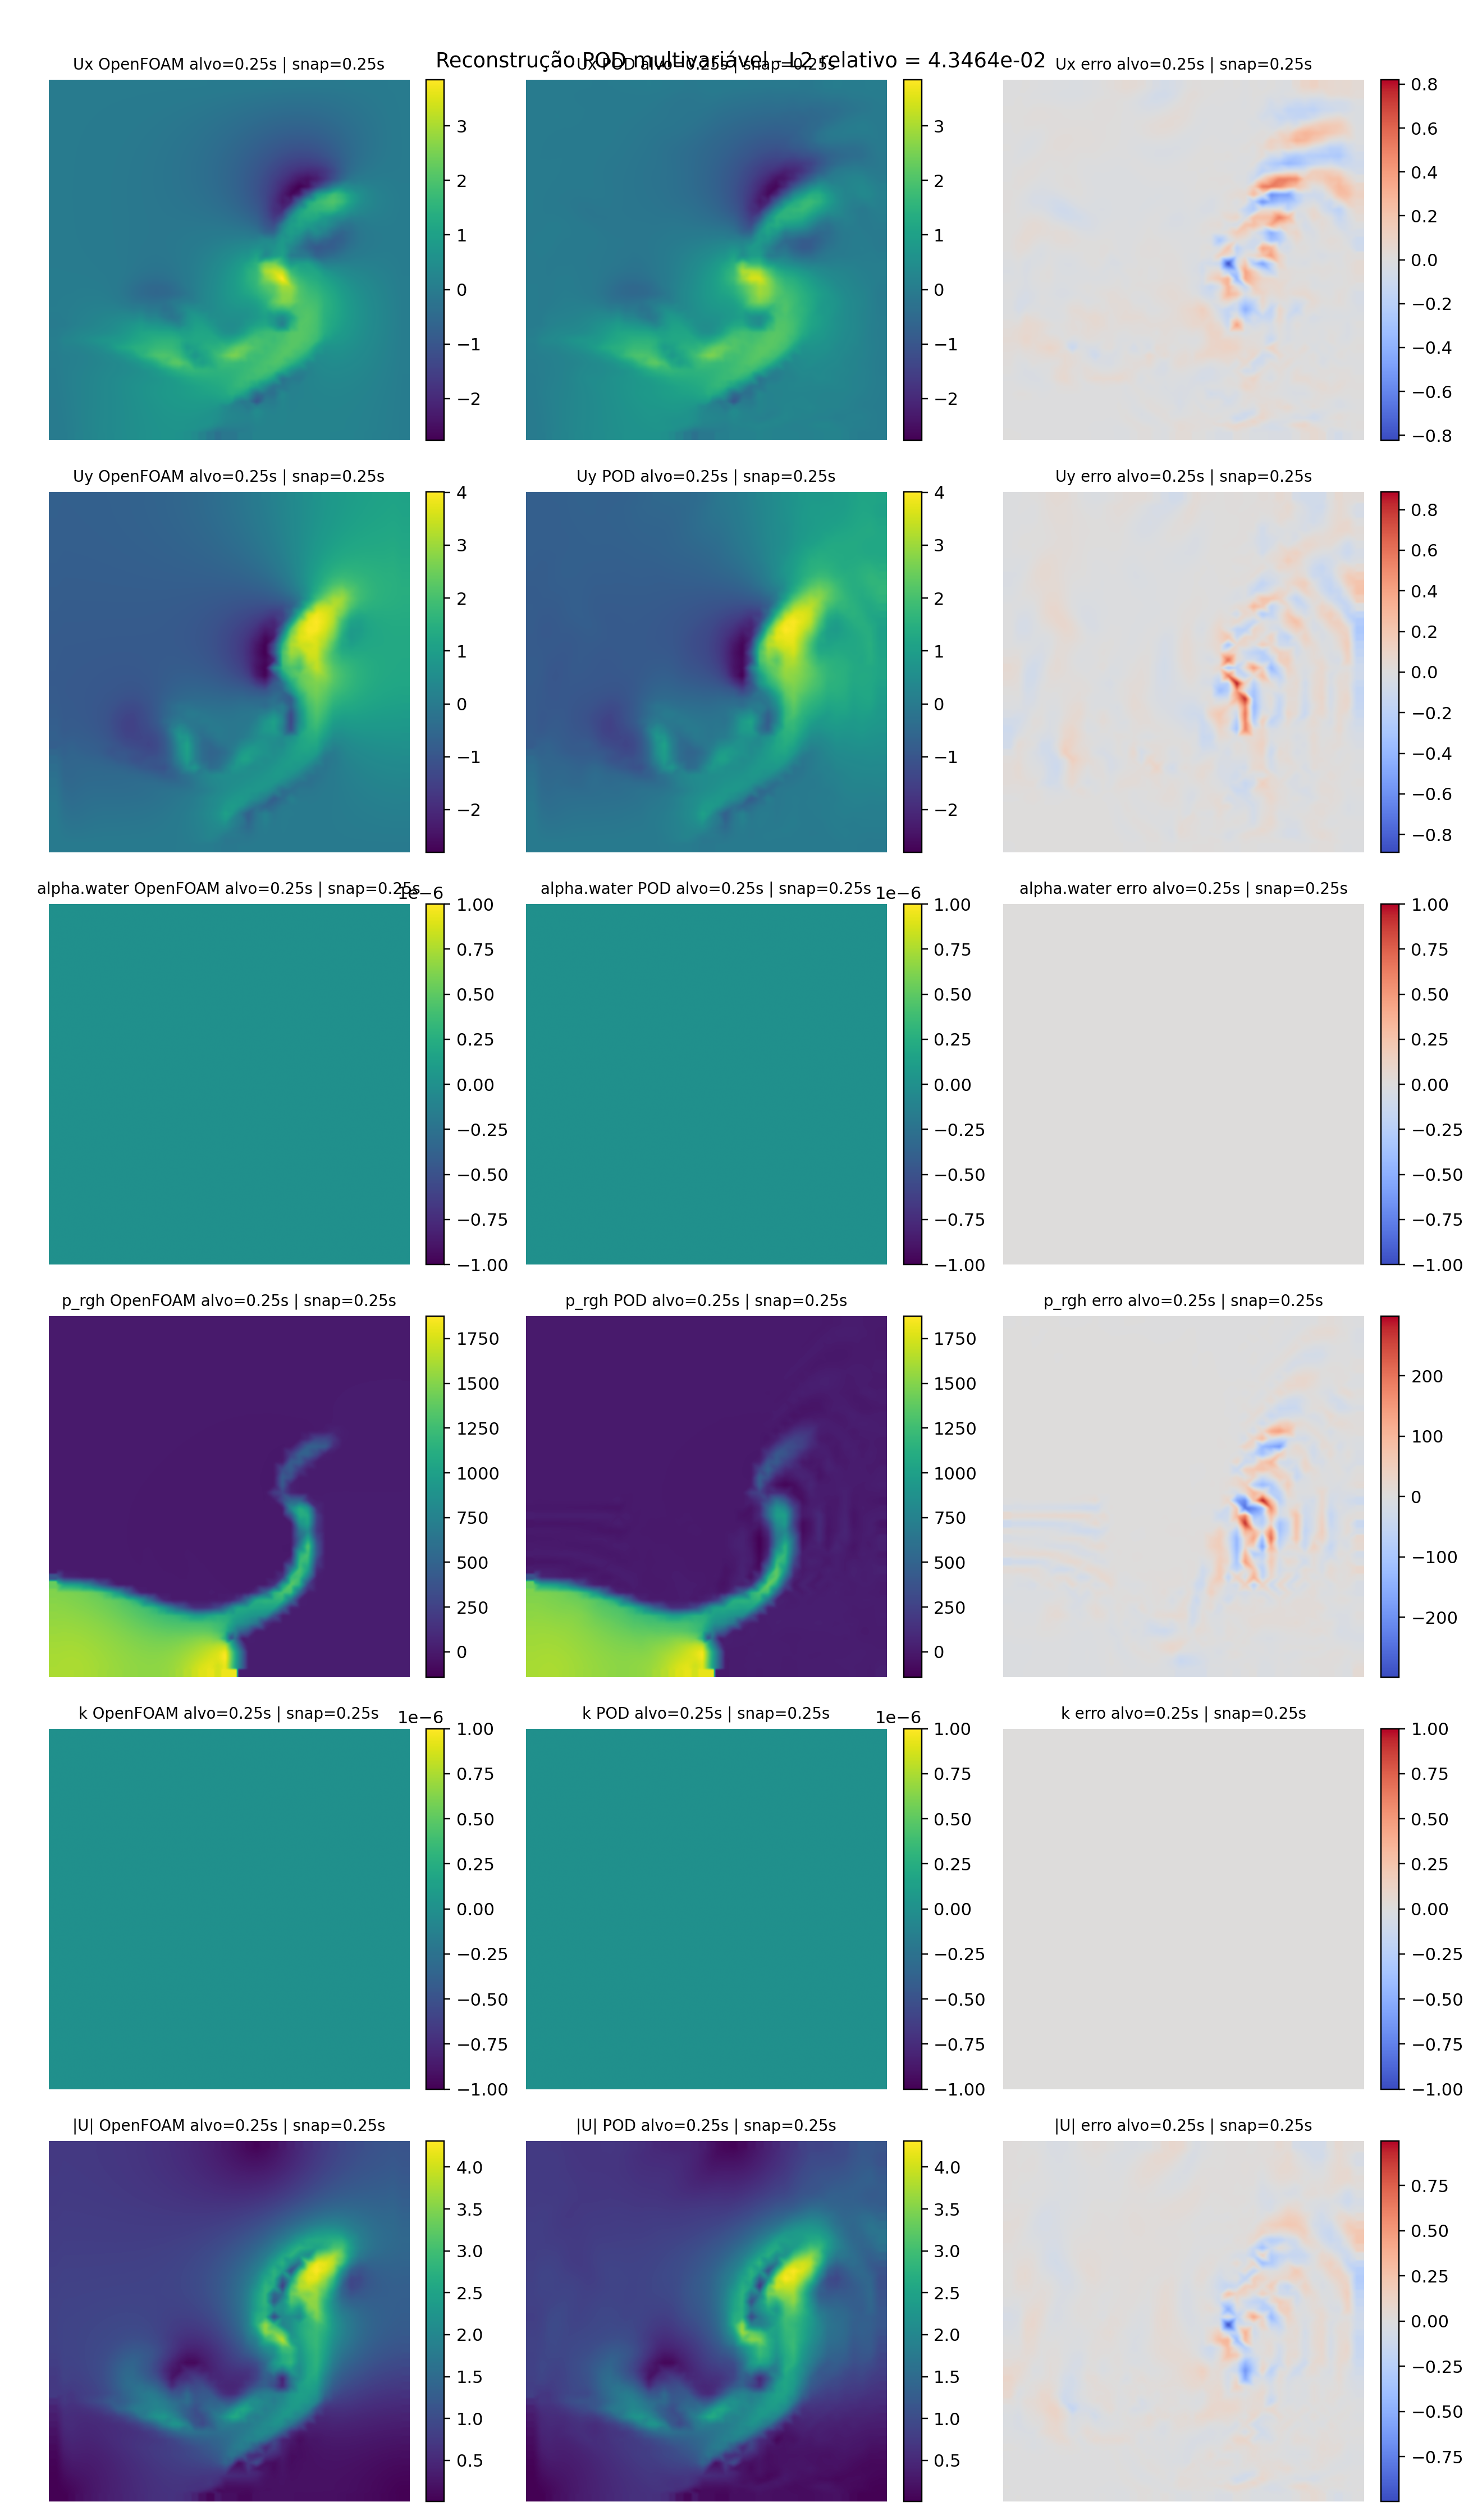
\includegraphics[height=.8\textheight,keepaspectratio]{pod_t025.png}\caption{Reconstrução POD isolada em $t=\SI{0.25}{s}$.}\end{figure}
\begin{figure}[H]\centering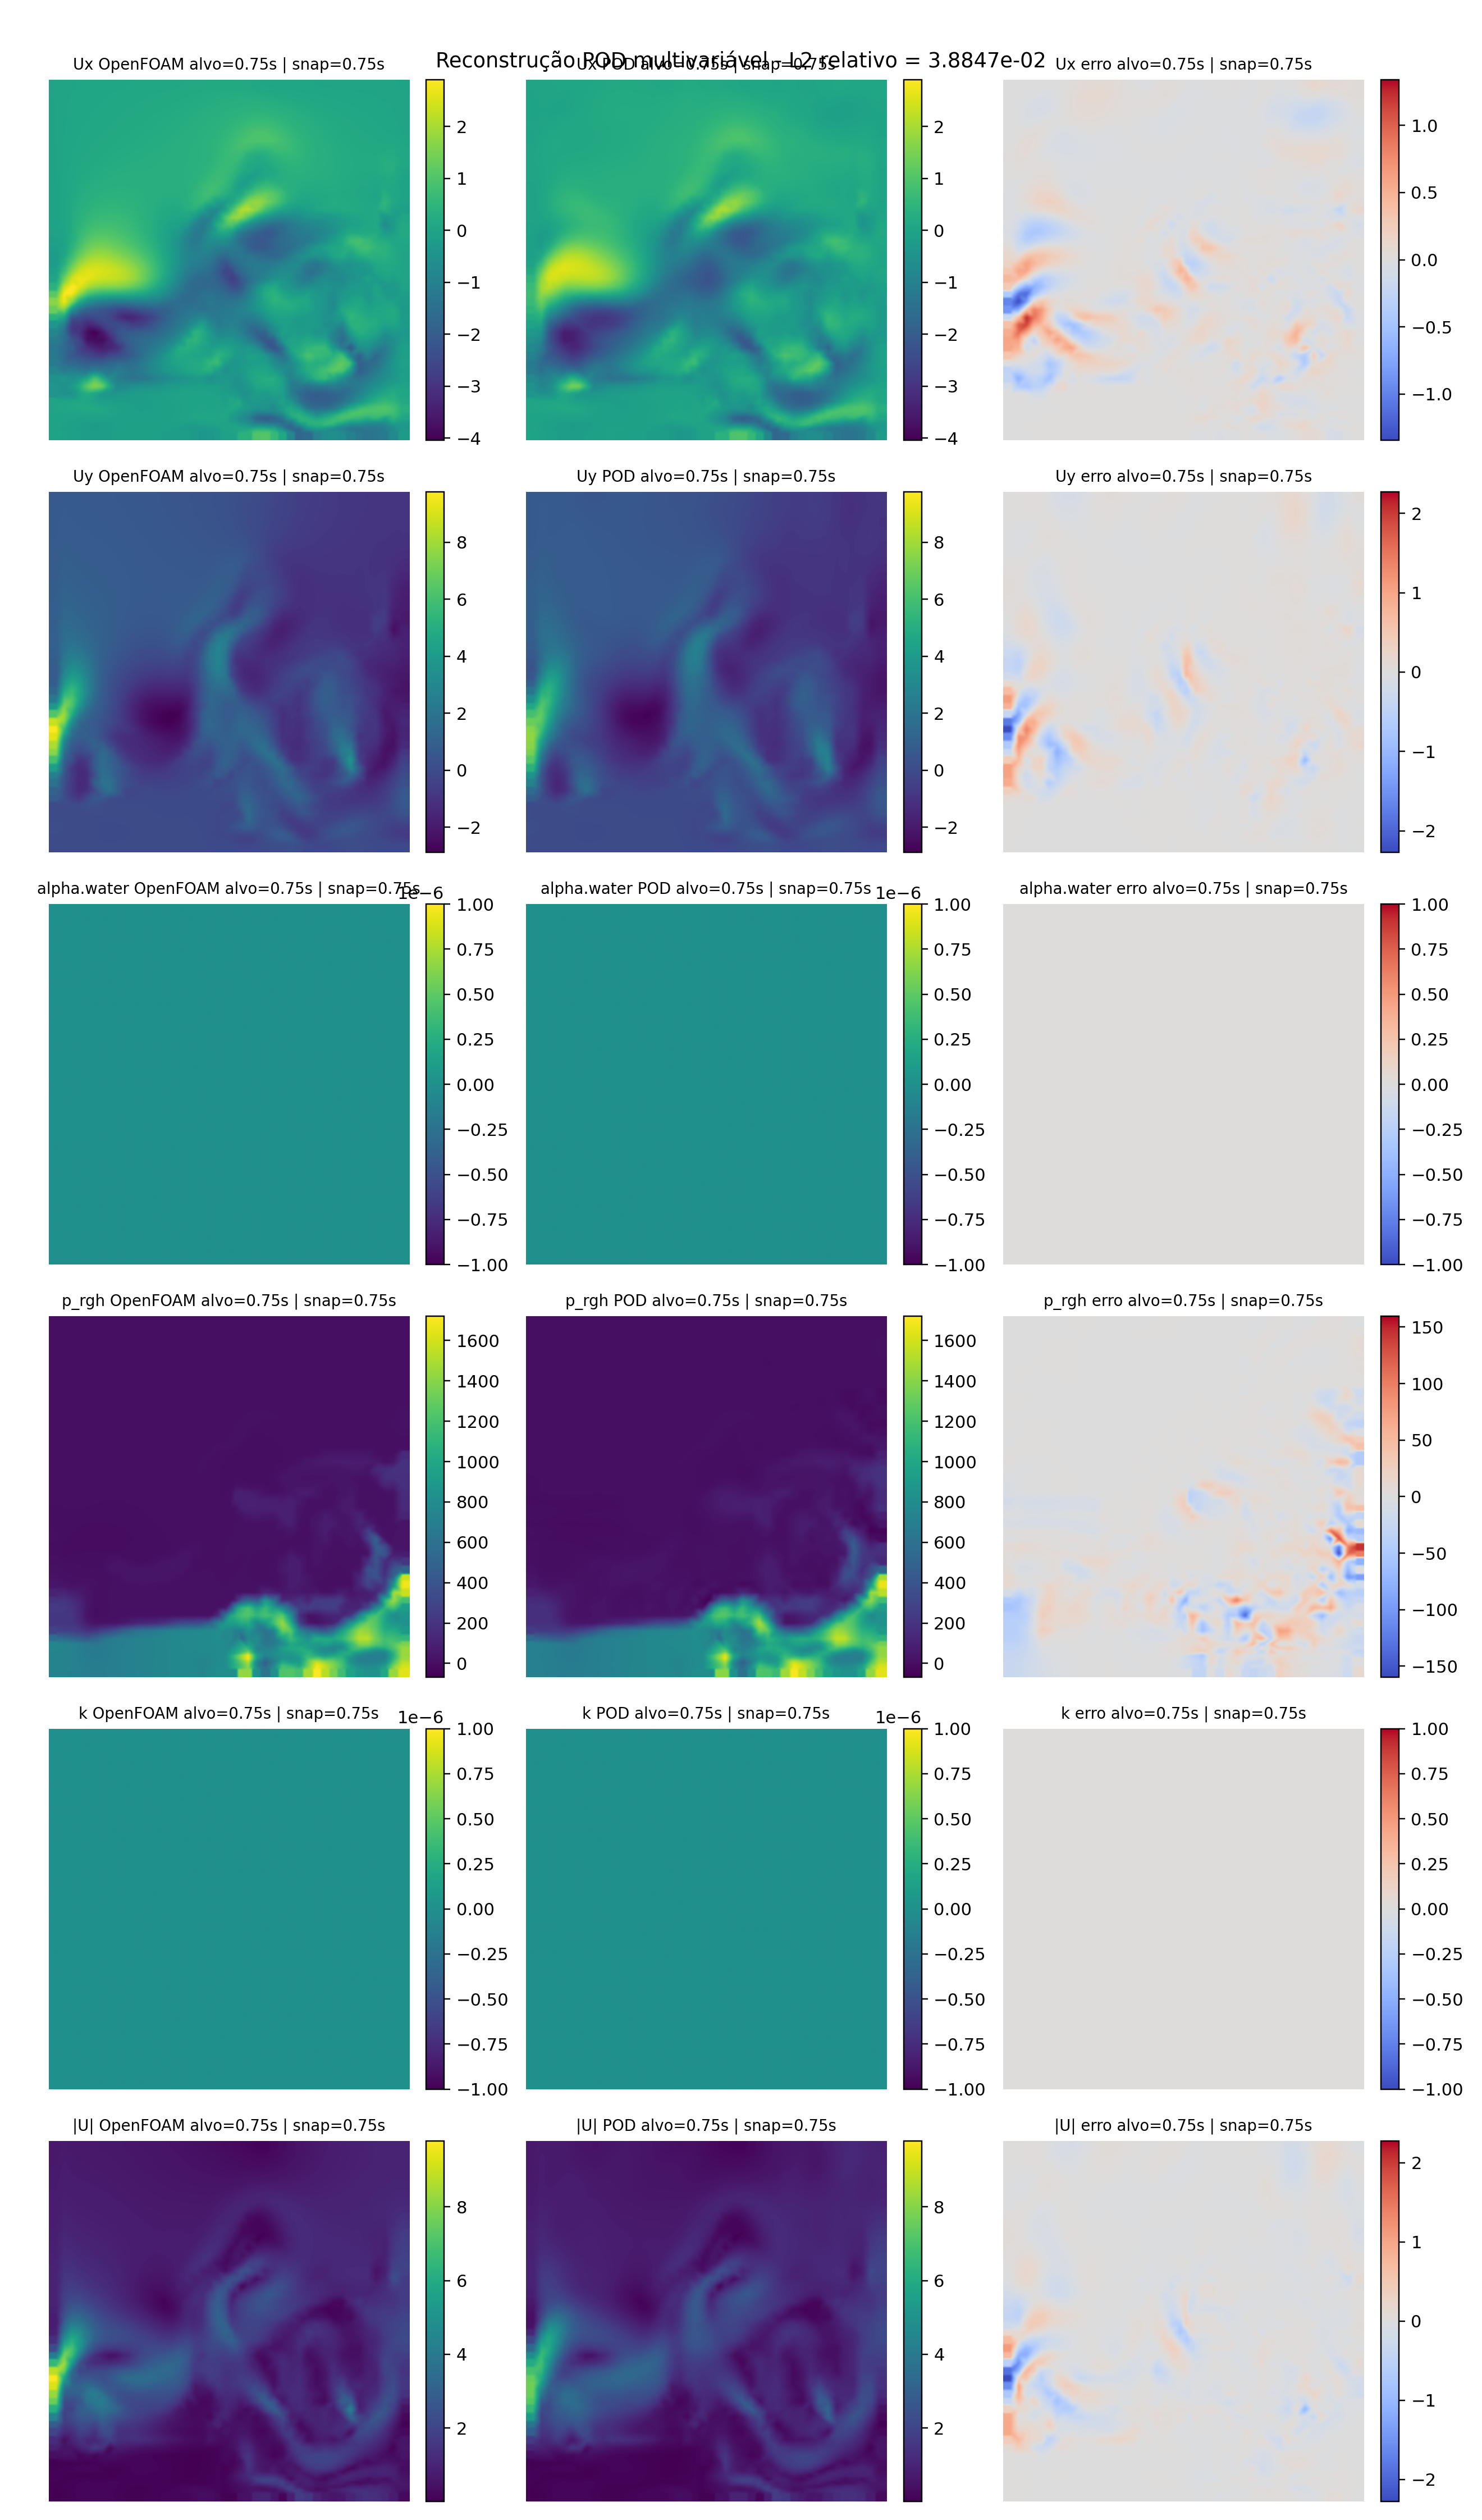
\includegraphics[height=.8\textheight,keepaspectratio]{pod_t075.png}\caption{Reconstrução POD isolada em $t=\SI{0.75}{s}$.}\end{figure}

A POD tem excelente reconstrução com 50 modos, mas oito modos---usados no primeiro SINDy---ainda deixam erro de projeção de 35,05\%. O canal $k$ nulo infla a descrição multivariável sem adicionar física.

\section{SAE multivariável}
O SAE usa grade $48\times48$, cinco canais e entrada de dimensão 11520. O encoder 128--64--32 leva a oito latentes lineares; o decoder é simétrico e emprega Batch Normalization. Foram usados Adam, taxa inicial $5\times10^{-5}$, Huber, lote 32, até 150 épocas, redução de taxa em platô e corte z-score $\pm4$. Dos 1001 snapshots amostrados com stride 10, os primeiros 801 ($t\le0,8$) treinam e os 200 finais validam.

\begin{table}[H]\centering\caption{Resultados SAE.}\label{tab:sae}
\begin{tabular}{lrr}\toprule Métrica&Treino&Validação\\\midrule
MSE médio&0,1467&2,4257\\Erro $L_2$ médio&0,4033&0,9176\\$R^2$ global&0,8221&0,1330\\\bottomrule\end{tabular}\end{table}
A melhor época é 47 e a menor perda de validação é 0,6633. O grande \emph{gap} indica que o SAE reconstrói o período visto, mas extrapola mal para $t>0,8\,\si{s}$. A densidade, derivada diretamente de $\alpha$, também introduz redundância entre canais.

\begin{figure}[H]\centering
\begin{subfigure}{.49\textwidth}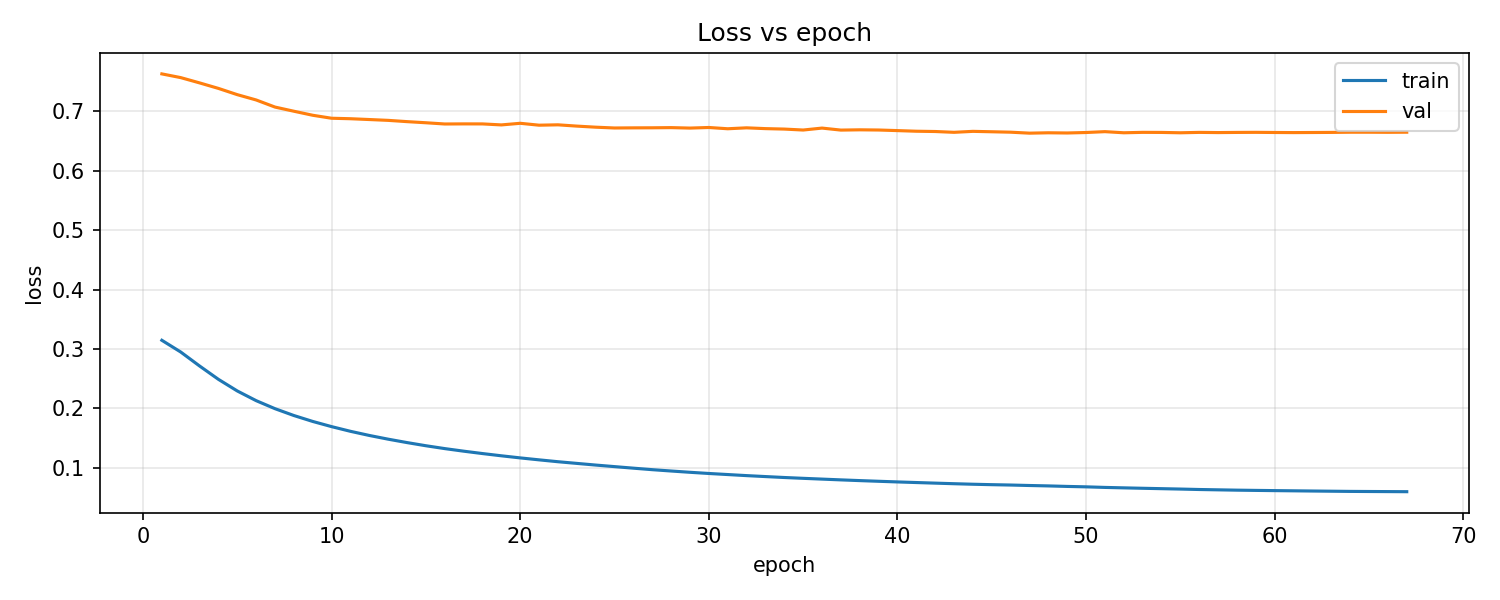
\includegraphics[width=\linewidth]{sae_loss.png}\caption{Perdas.}\end{subfigure}
\begin{subfigure}{.49\textwidth}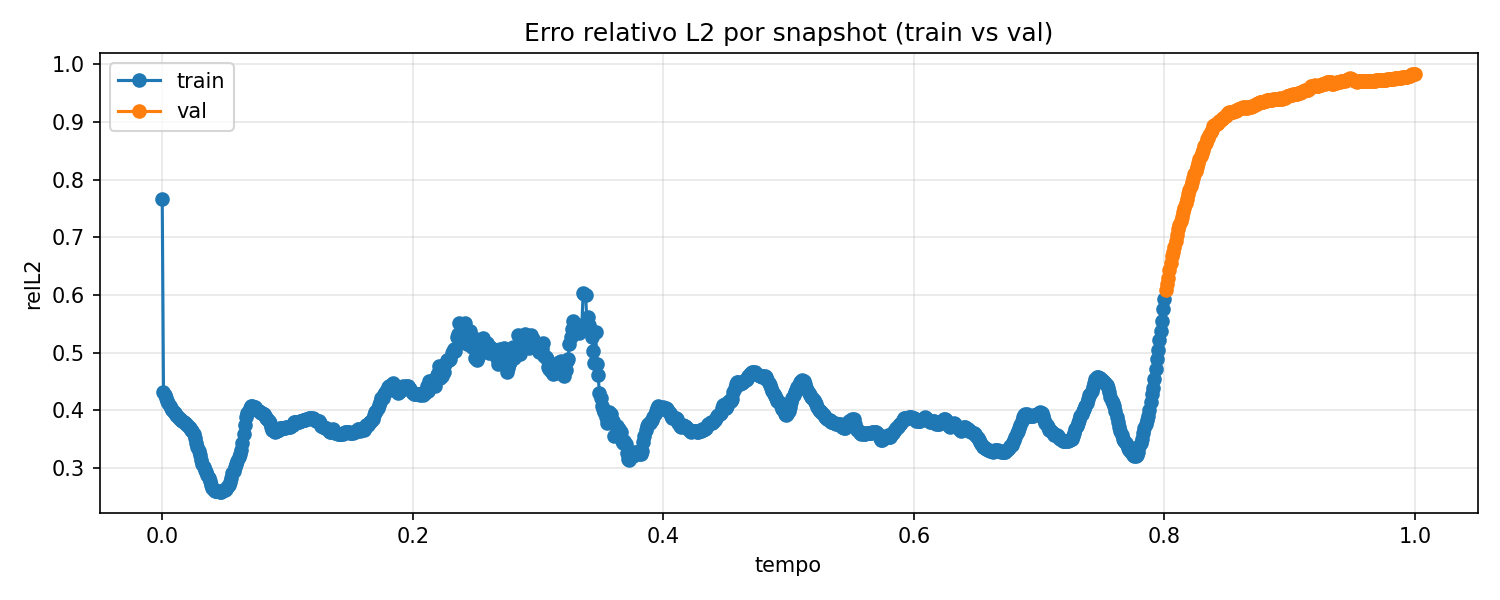
\includegraphics[width=\linewidth]{sae_rel.png}\caption{Erro por snapshot.}\end{subfigure}
\caption{Diagnóstico SAE.}\end{figure}
\begin{figure}[H]\centering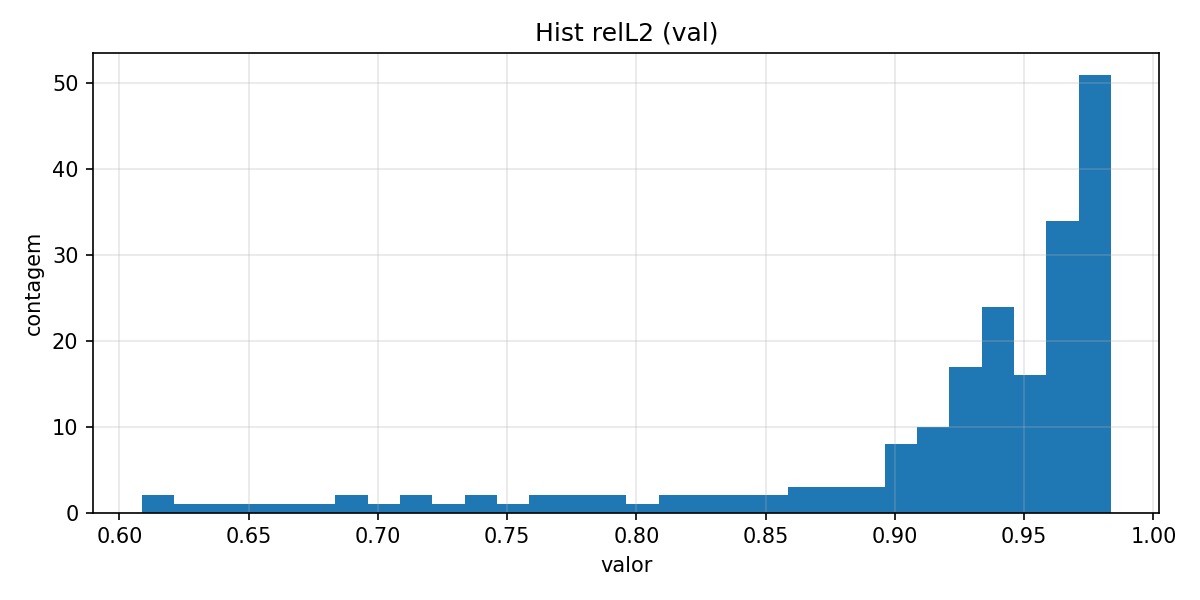
\includegraphics[width=.62\textwidth]{sae_hist.png}\caption{Erro relativo de validação.}\end{figure}
\begin{figure}[H]\centering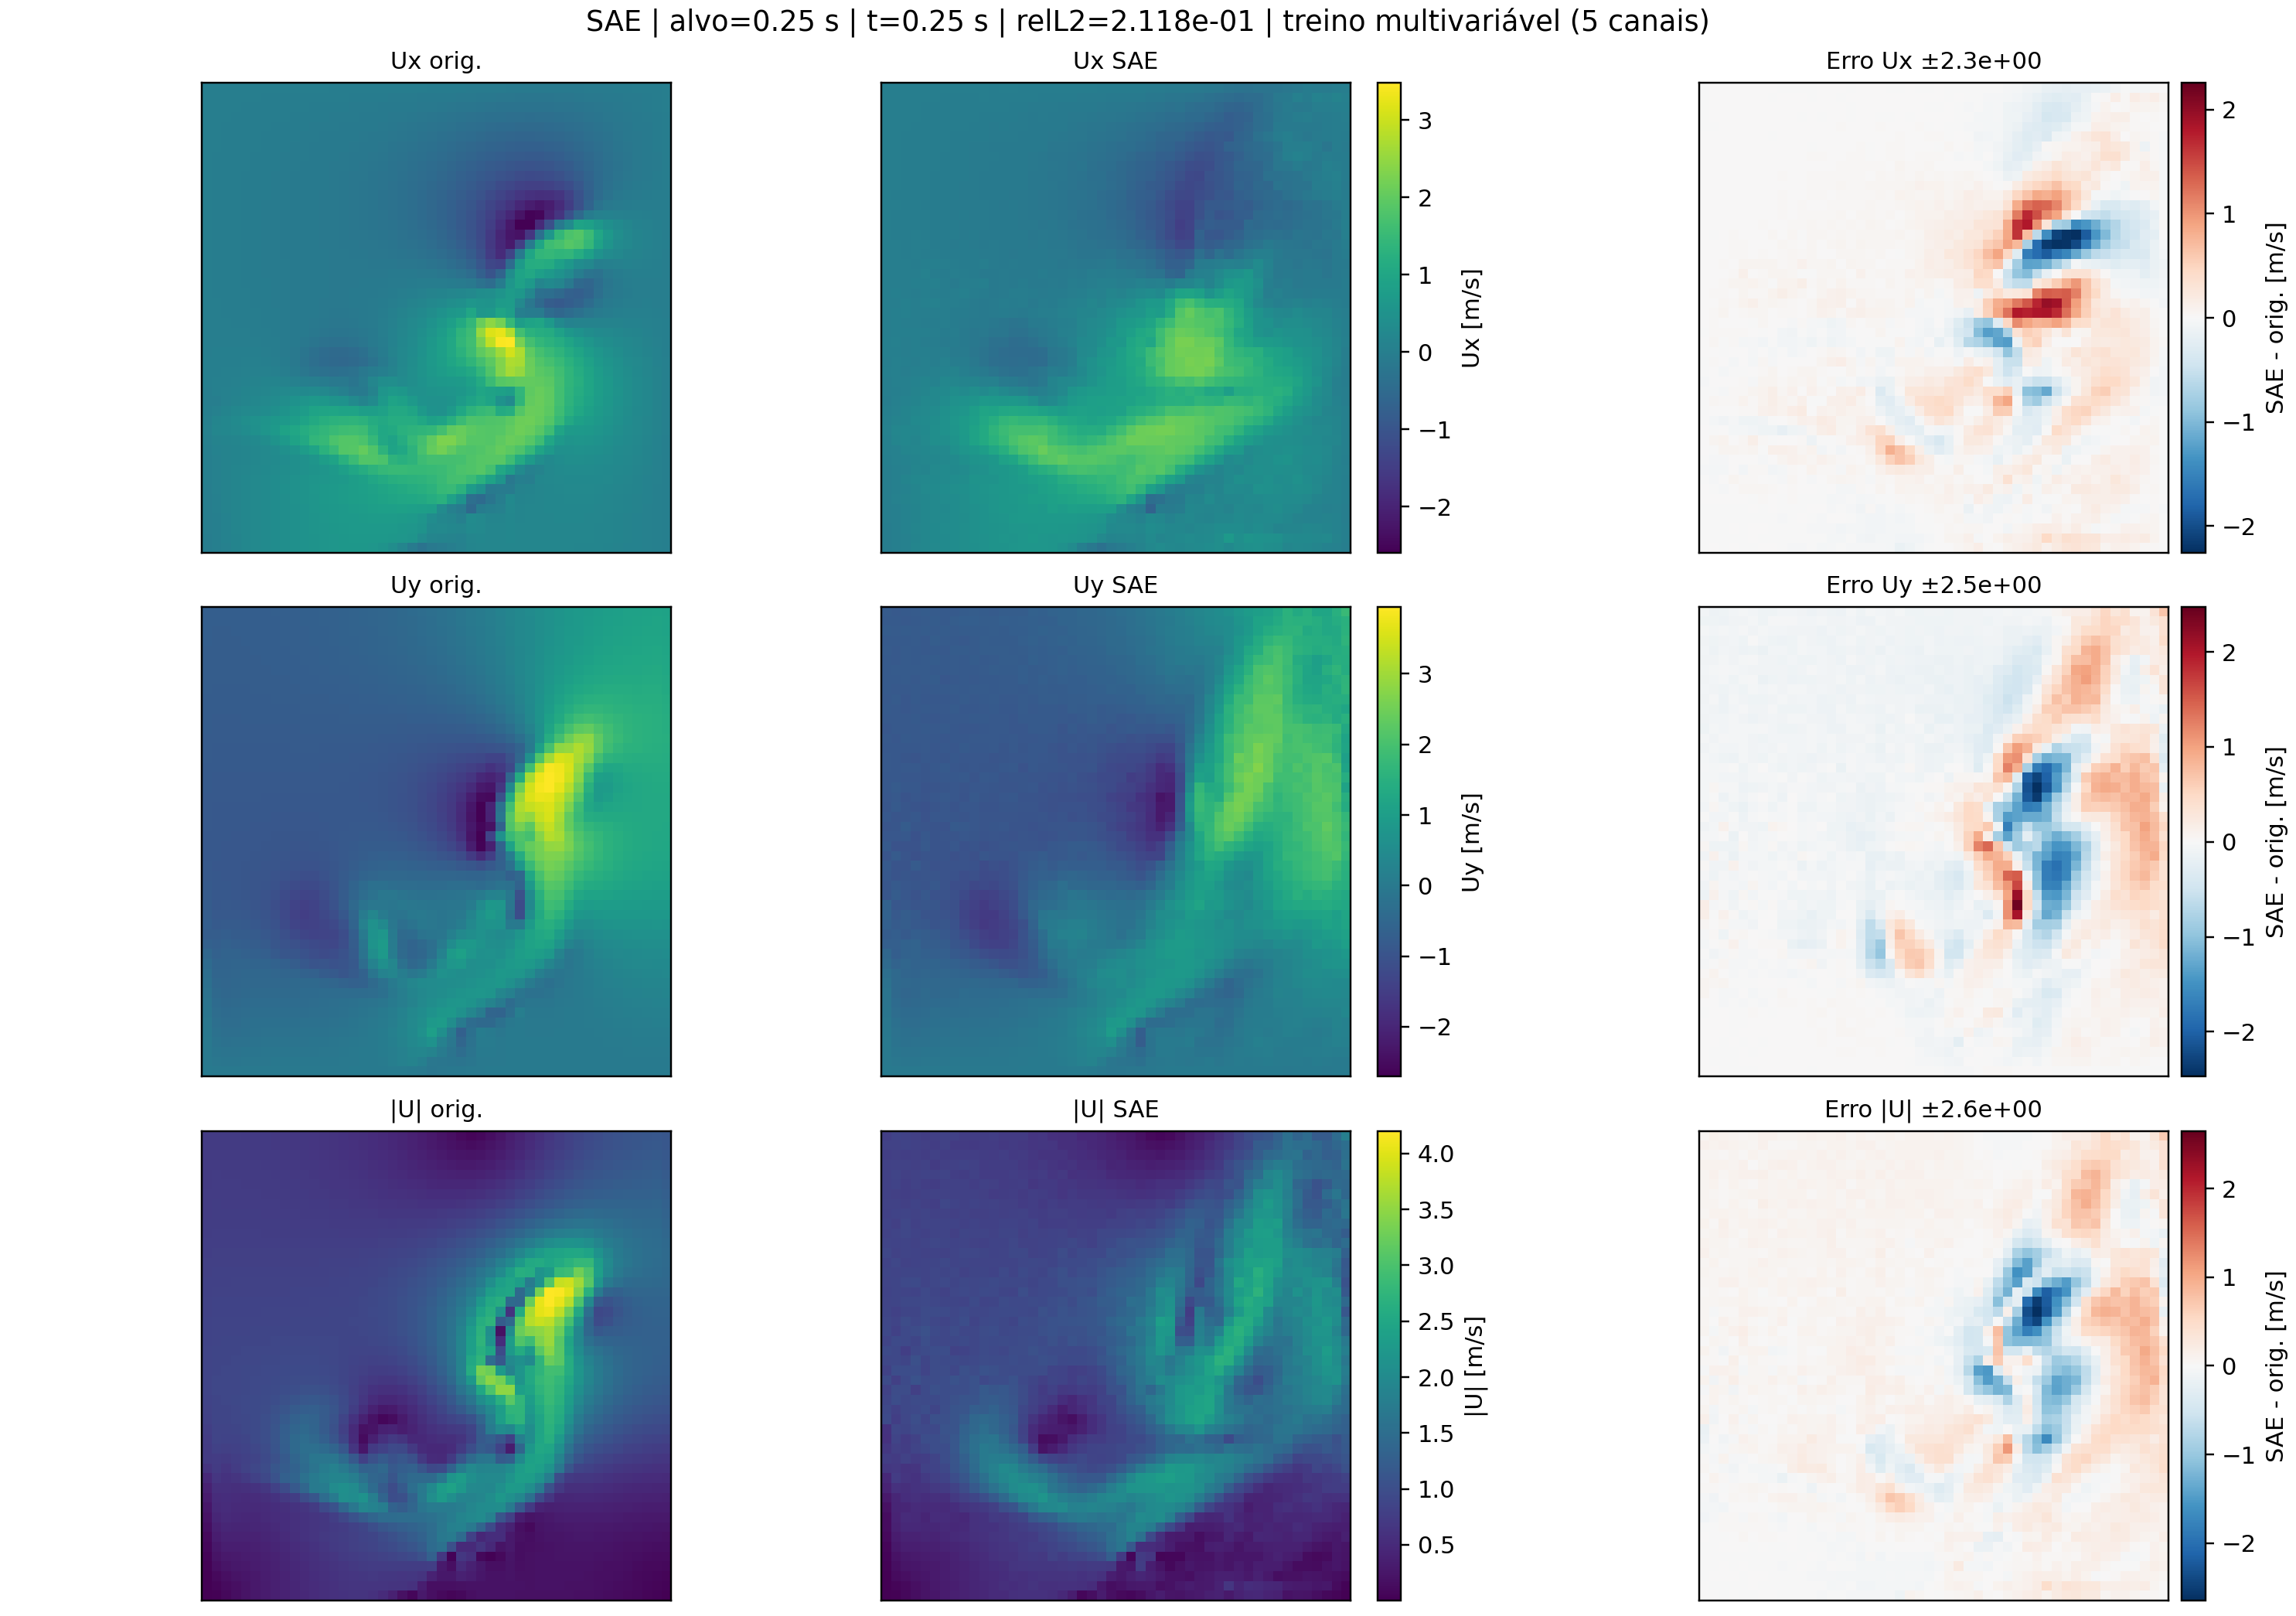
\includegraphics[width=.92\textwidth]{sae_t025.png}\caption{Reconstrução SAE isolada em $t=\SI{0.25}{s}$.}\end{figure}
\begin{figure}[H]\centering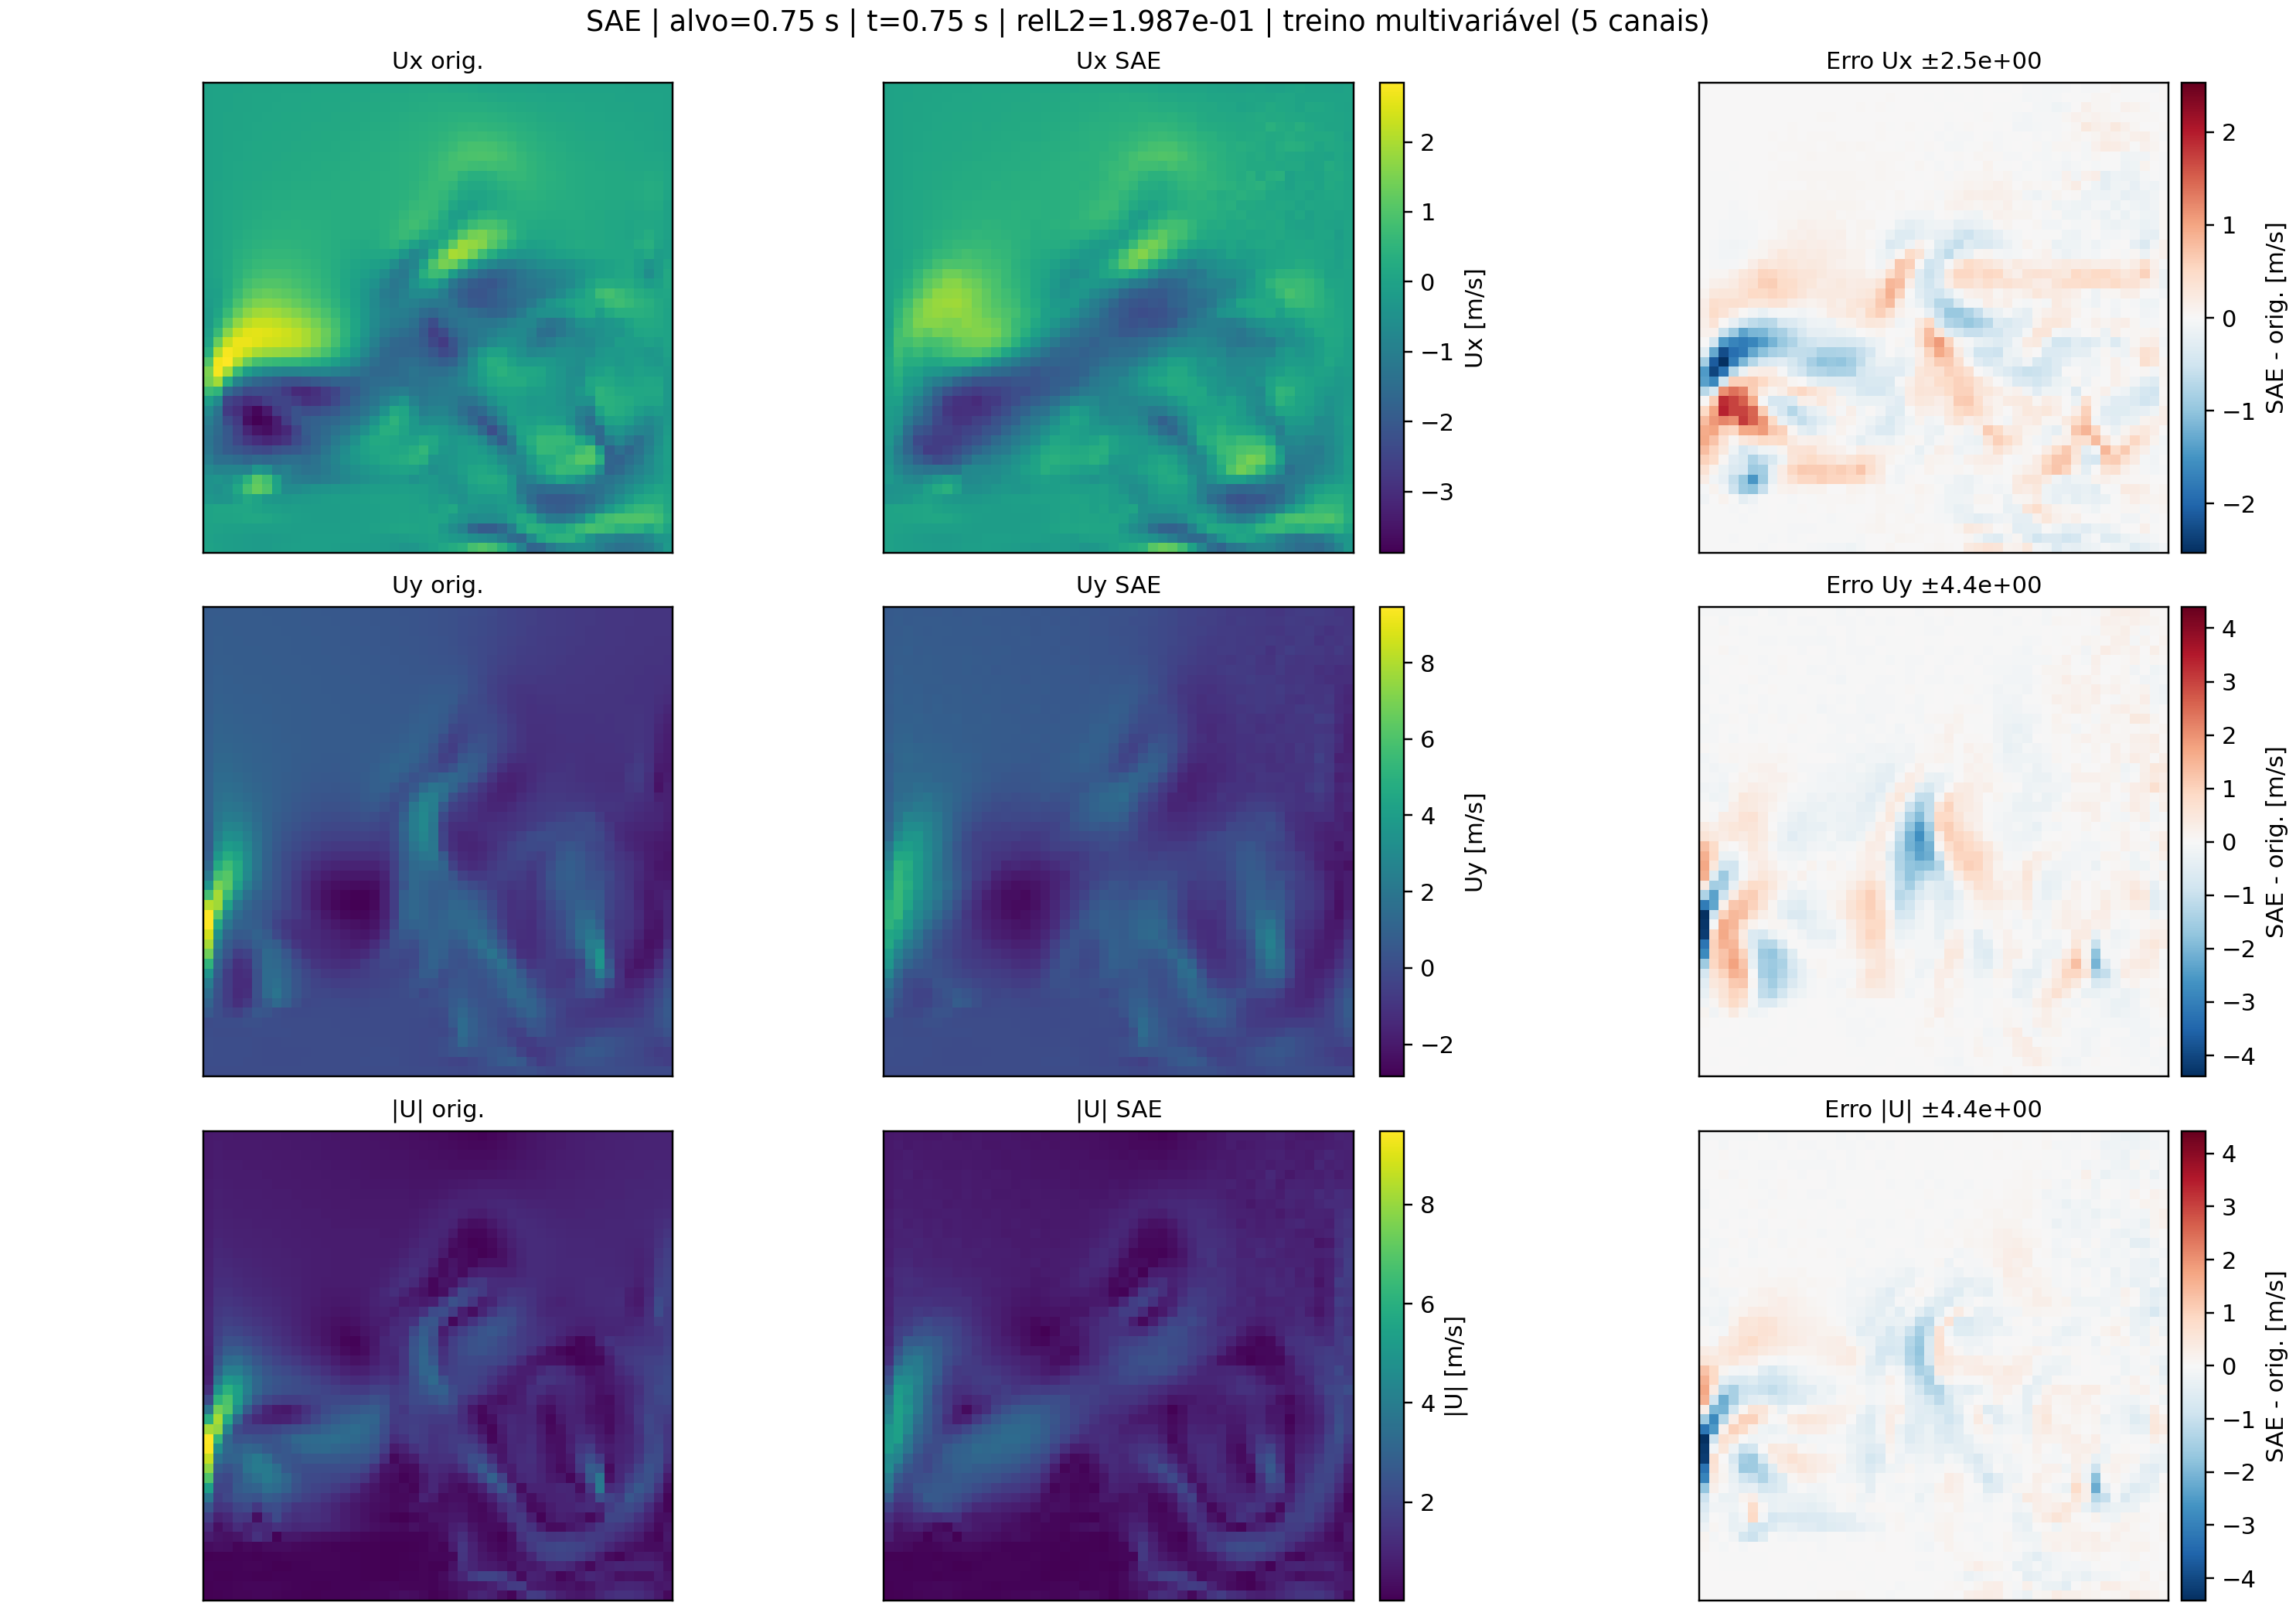
\includegraphics[width=.92\textwidth]{sae_t075.png}\caption{Reconstrução SAE em $t=\SI{0.75}{s}$.}\end{figure}

POD e SAE isolados são redutores/reconstrutores: nenhuma dessas etapas contém uma equação de evolução. Logo, energia, MSE e $R^2$ de reconstrução medem representação dos dados, não captura dinâmica.

\section{SINDy e equações descobertas}
SINDy identifica $\dot q=\Theta(q,t)\Xi$. A integração livre é o teste decisivo; erros de derivada ou de um passo podem ser pequenos mesmo quando a trajetória autônoma é instável.

\subsection{POD--SINDy}
O modelo principal usa oito modos, ordem 2 sem seno e biblioteca de 45 termos. Embora o melhor ajuste de derivada tenha ocorrido em $\alpha=10^{-4}$, foi selecionado $\alpha=0,1$ para estabilidade/parcimônia: 16 termos não nulos em 360 possíveis, erro de derivada 0,2524. A integração livre falhou; o erro reportado 1,4645 é de fallback guiado e já é elevado.
\lstinputlisting[style=sindyeq,caption={Equações completas POD--SINDy.}]{equacoes_pod_sindy.txt}
\begin{figure}[H]\centering
\begin{subfigure}{.49\textwidth}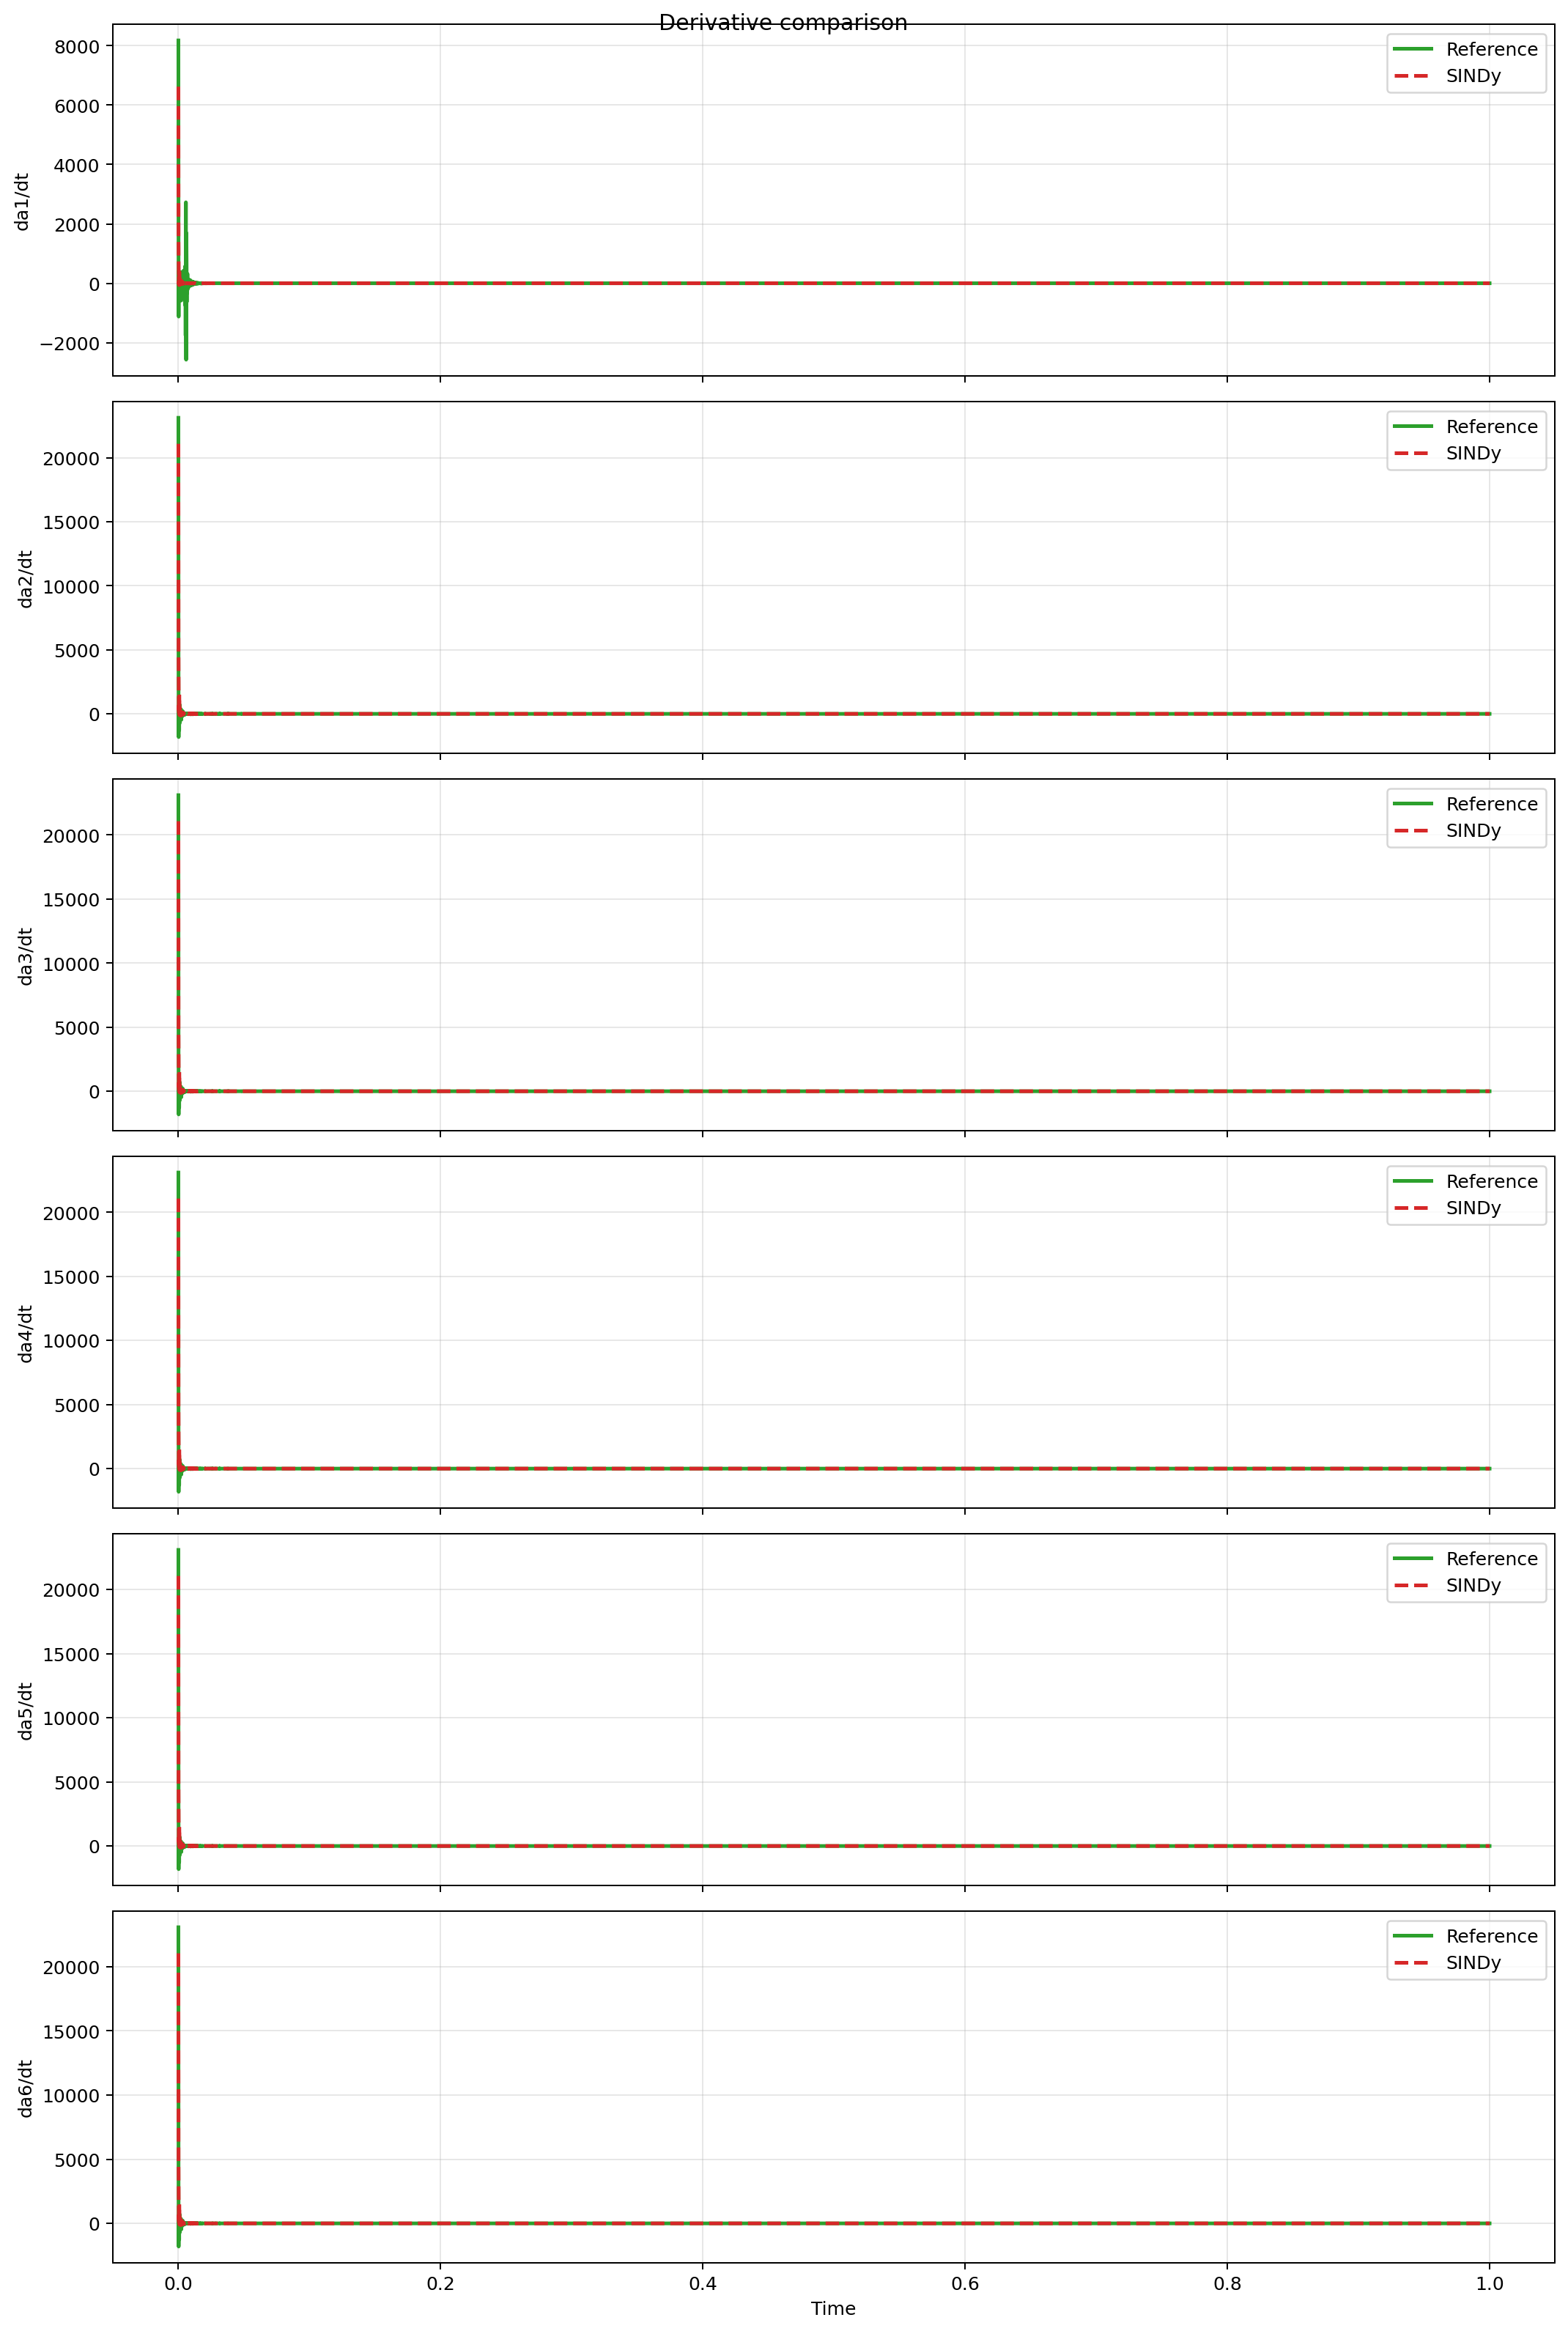
\includegraphics[width=\linewidth]{pods_deriv.png}\caption{Derivadas.}\end{subfigure}
\begin{subfigure}{.49\textwidth}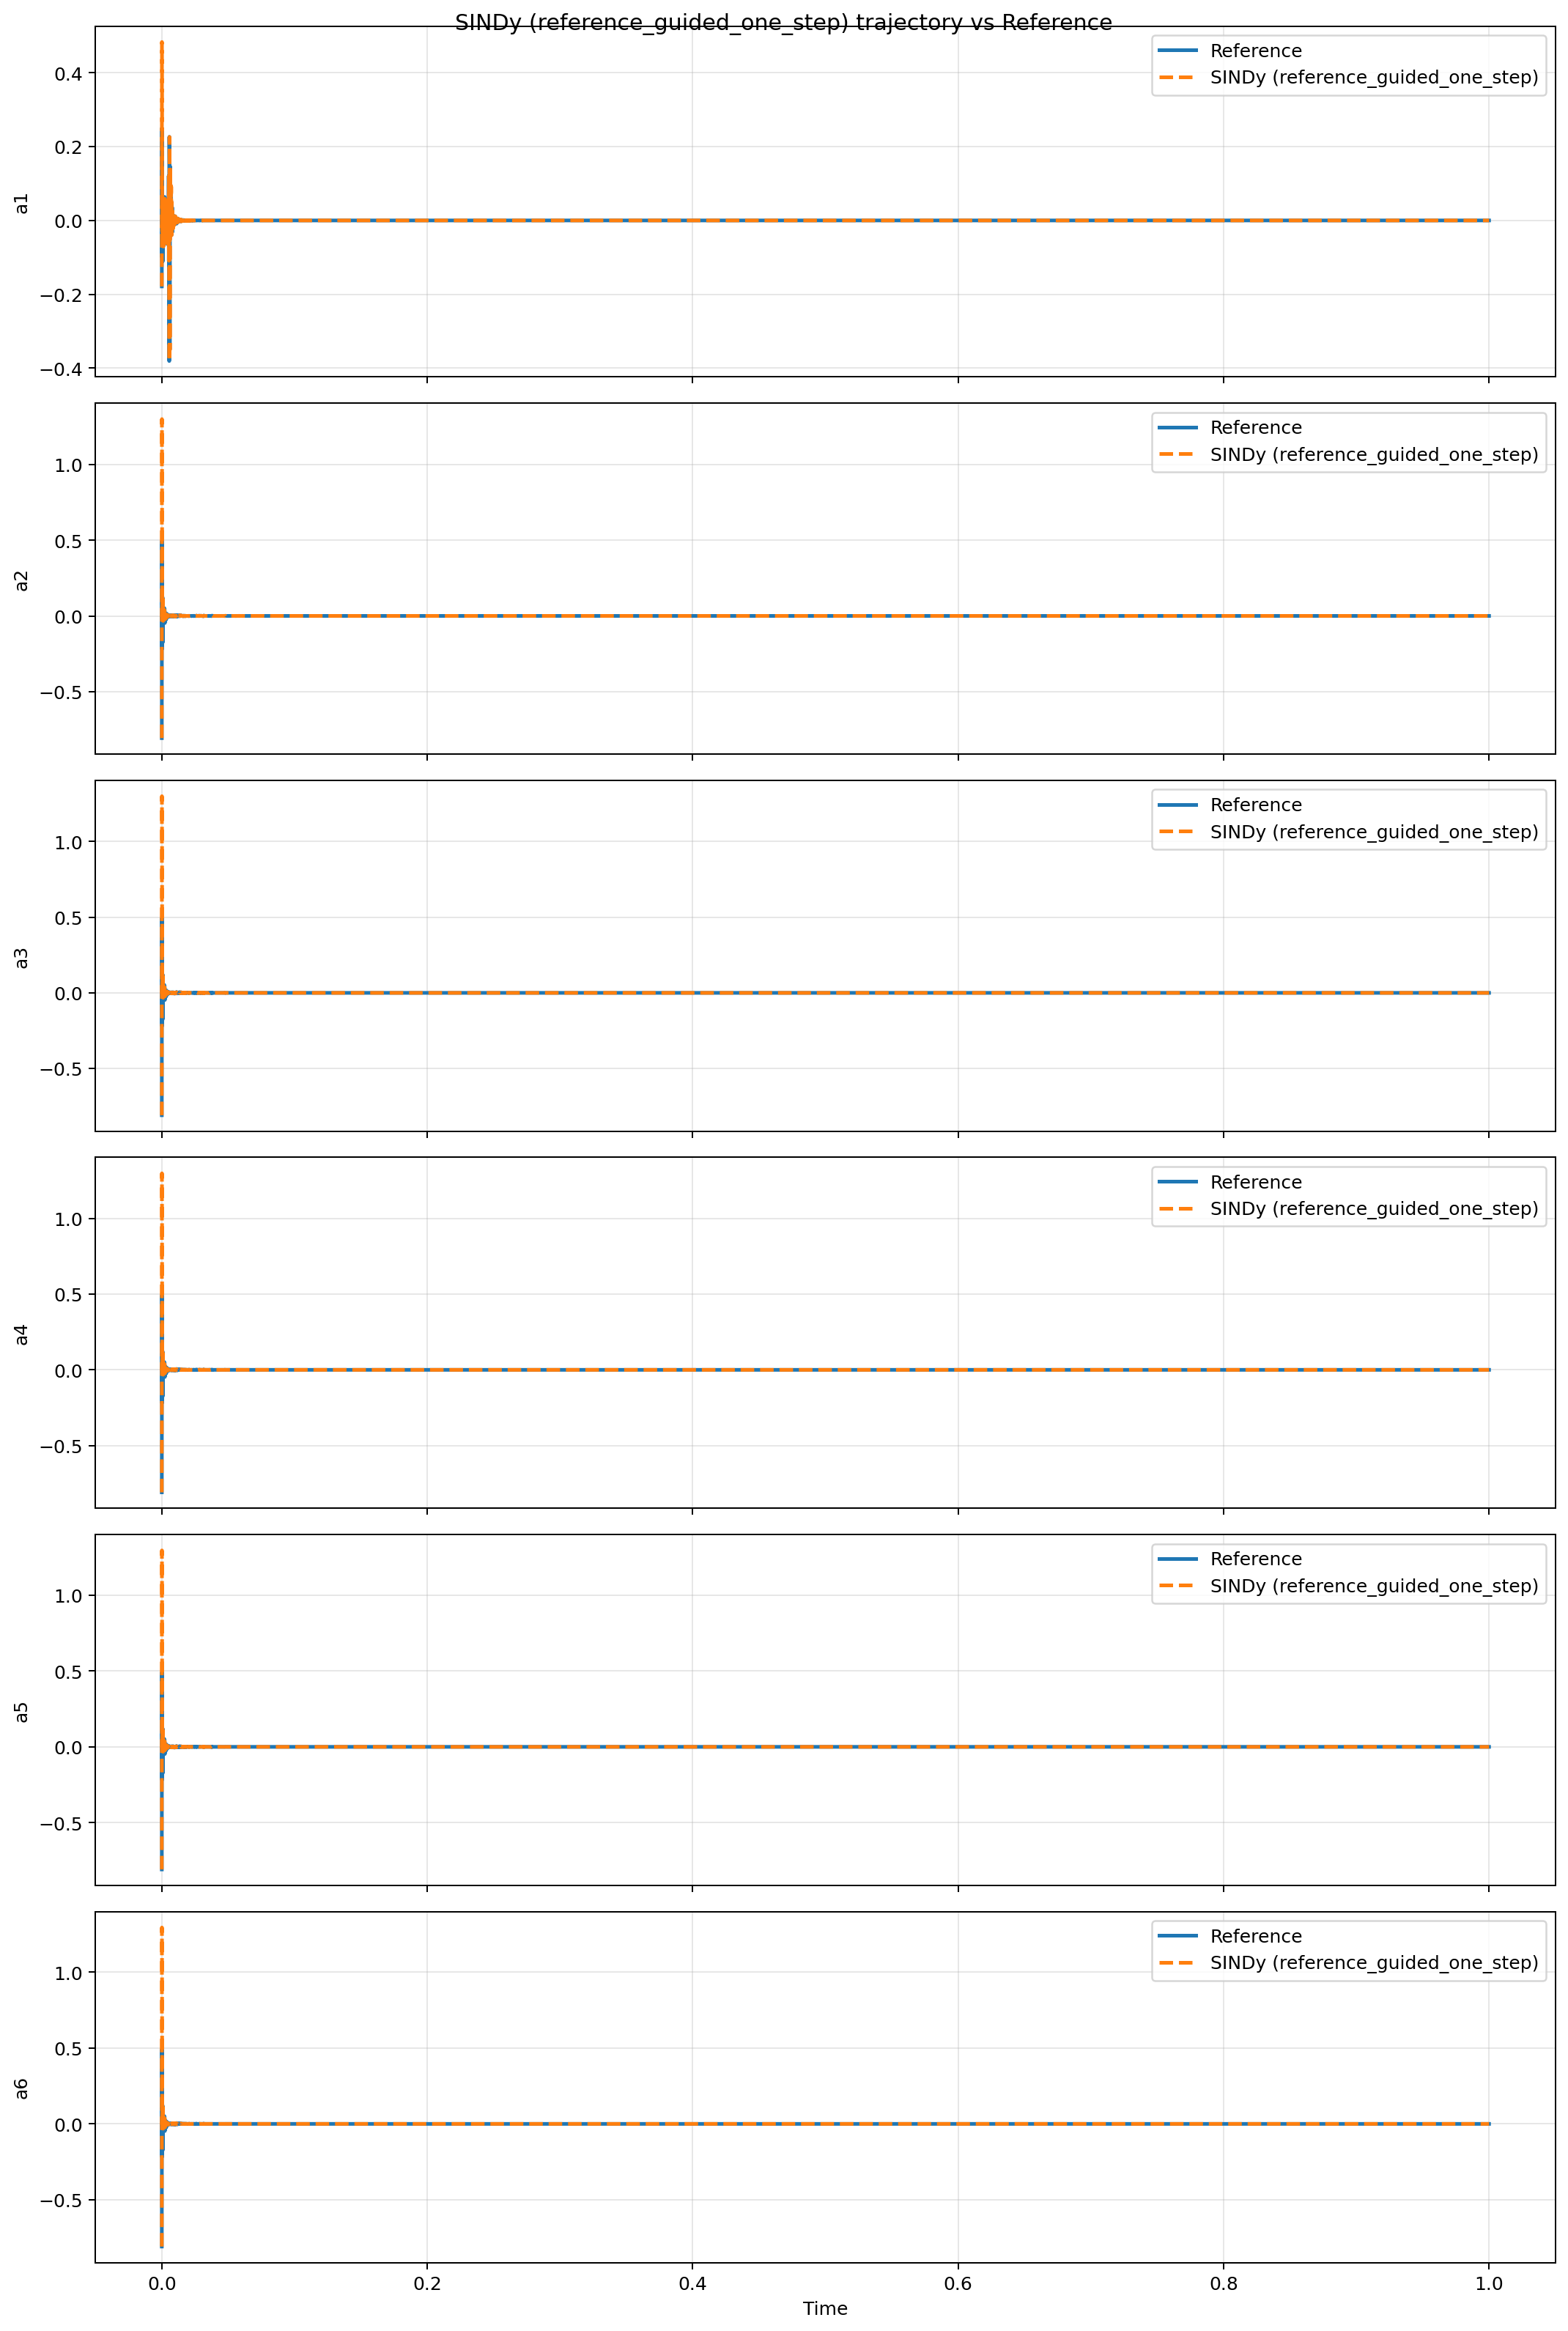
\includegraphics[width=\linewidth]{pods_traj.png}\caption{Trajetória guiada.}\end{subfigure}
\caption{POD--SINDy.}\end{figure}
\begin{figure}[H]\centering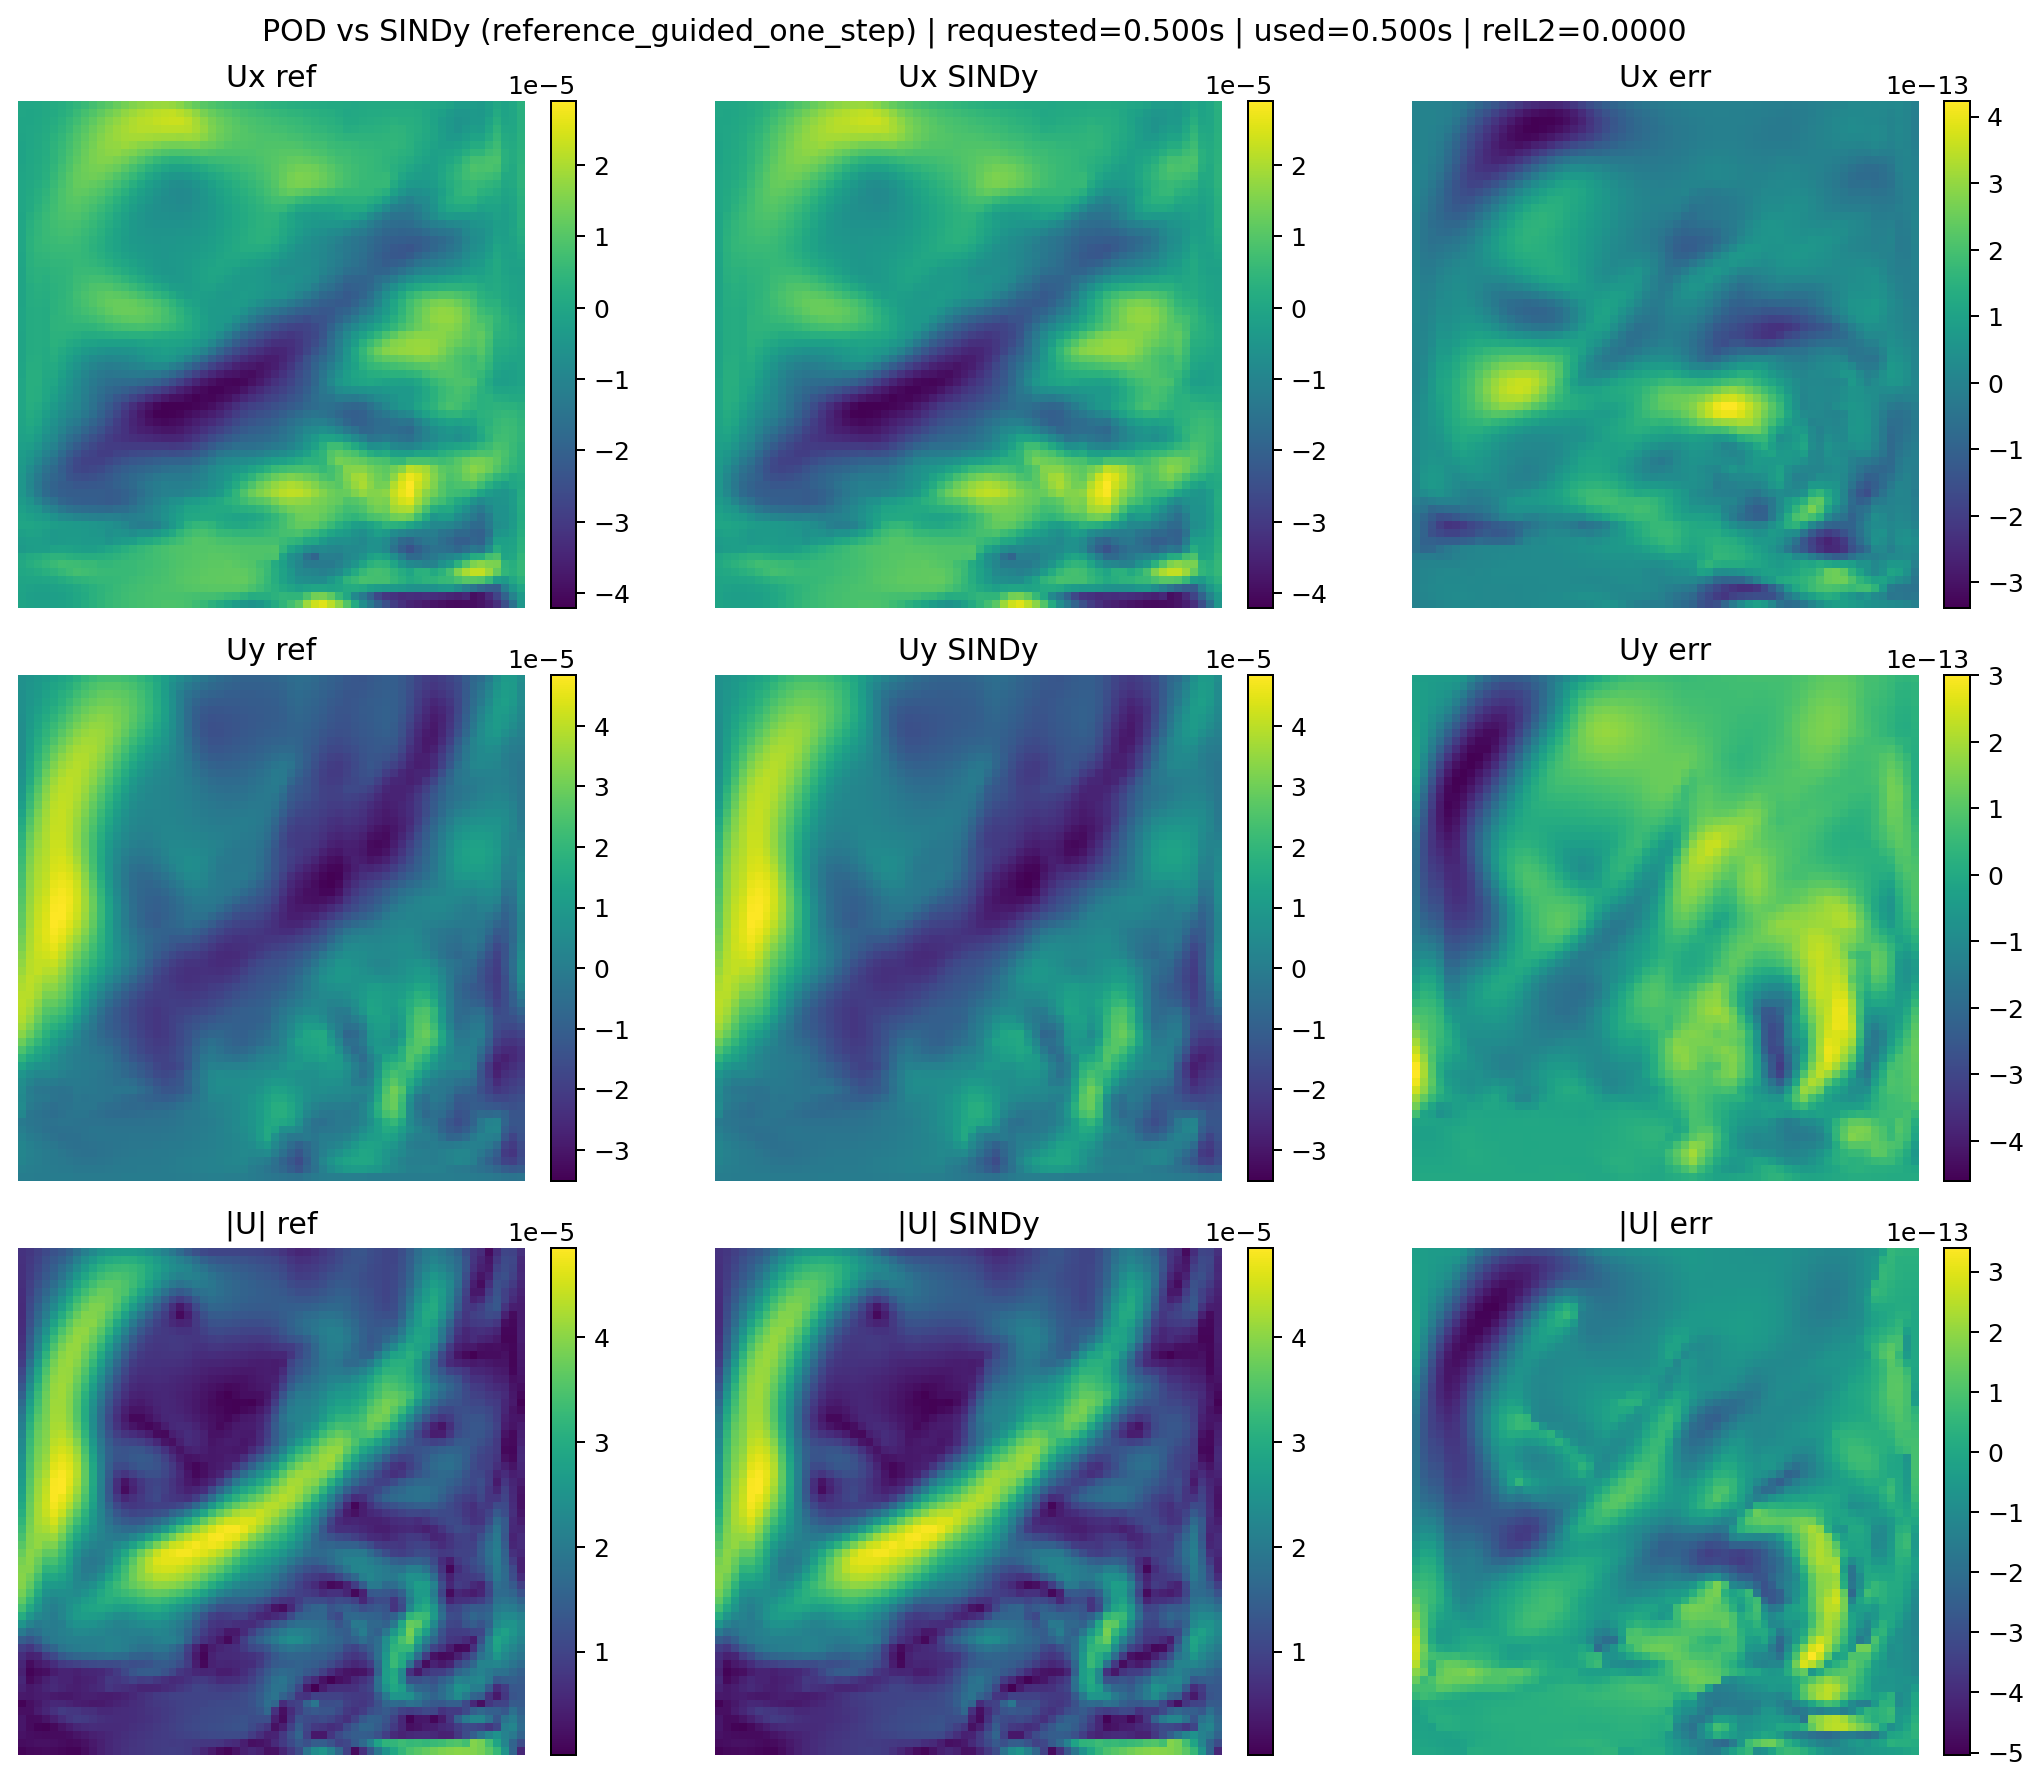
\includegraphics[width=.9\textwidth]{pods_t05.png}\caption{Campo POD--SINDy em $t=\SI{0.5}{s}$.}\end{figure}

A busca posterior não aceitou nenhum dos 84 modelos. O melhor compromisso usa 16 modos (94,94\% de energia), ordem 1, sem seno, $\alpha=0,1$, 31 termos em 272, erro de derivada 0,7132 e erro livre 0,7827. A integração funciona nessa alternativa, mas a precisão permanece insuficiente.

\subsection{SAE--SINDy}
Com oito latentes, ordem 2, seno/cosseno e 61 funções por equação, Lasso $\alpha=10^{-3}$ mantém 428 de 488 coeficientes. O erro de derivada é 0,7078. A integração livre falha; o erro guiado 0,0354 não deve ser interpretado como previsão autônoma.
\lstinputlisting[style=sindyeq,caption={Equações completas SAE--SINDy.}]{equacoes_sae_sindy.txt}
\begin{figure}[H]\centering
\begin{subfigure}{.49\textwidth}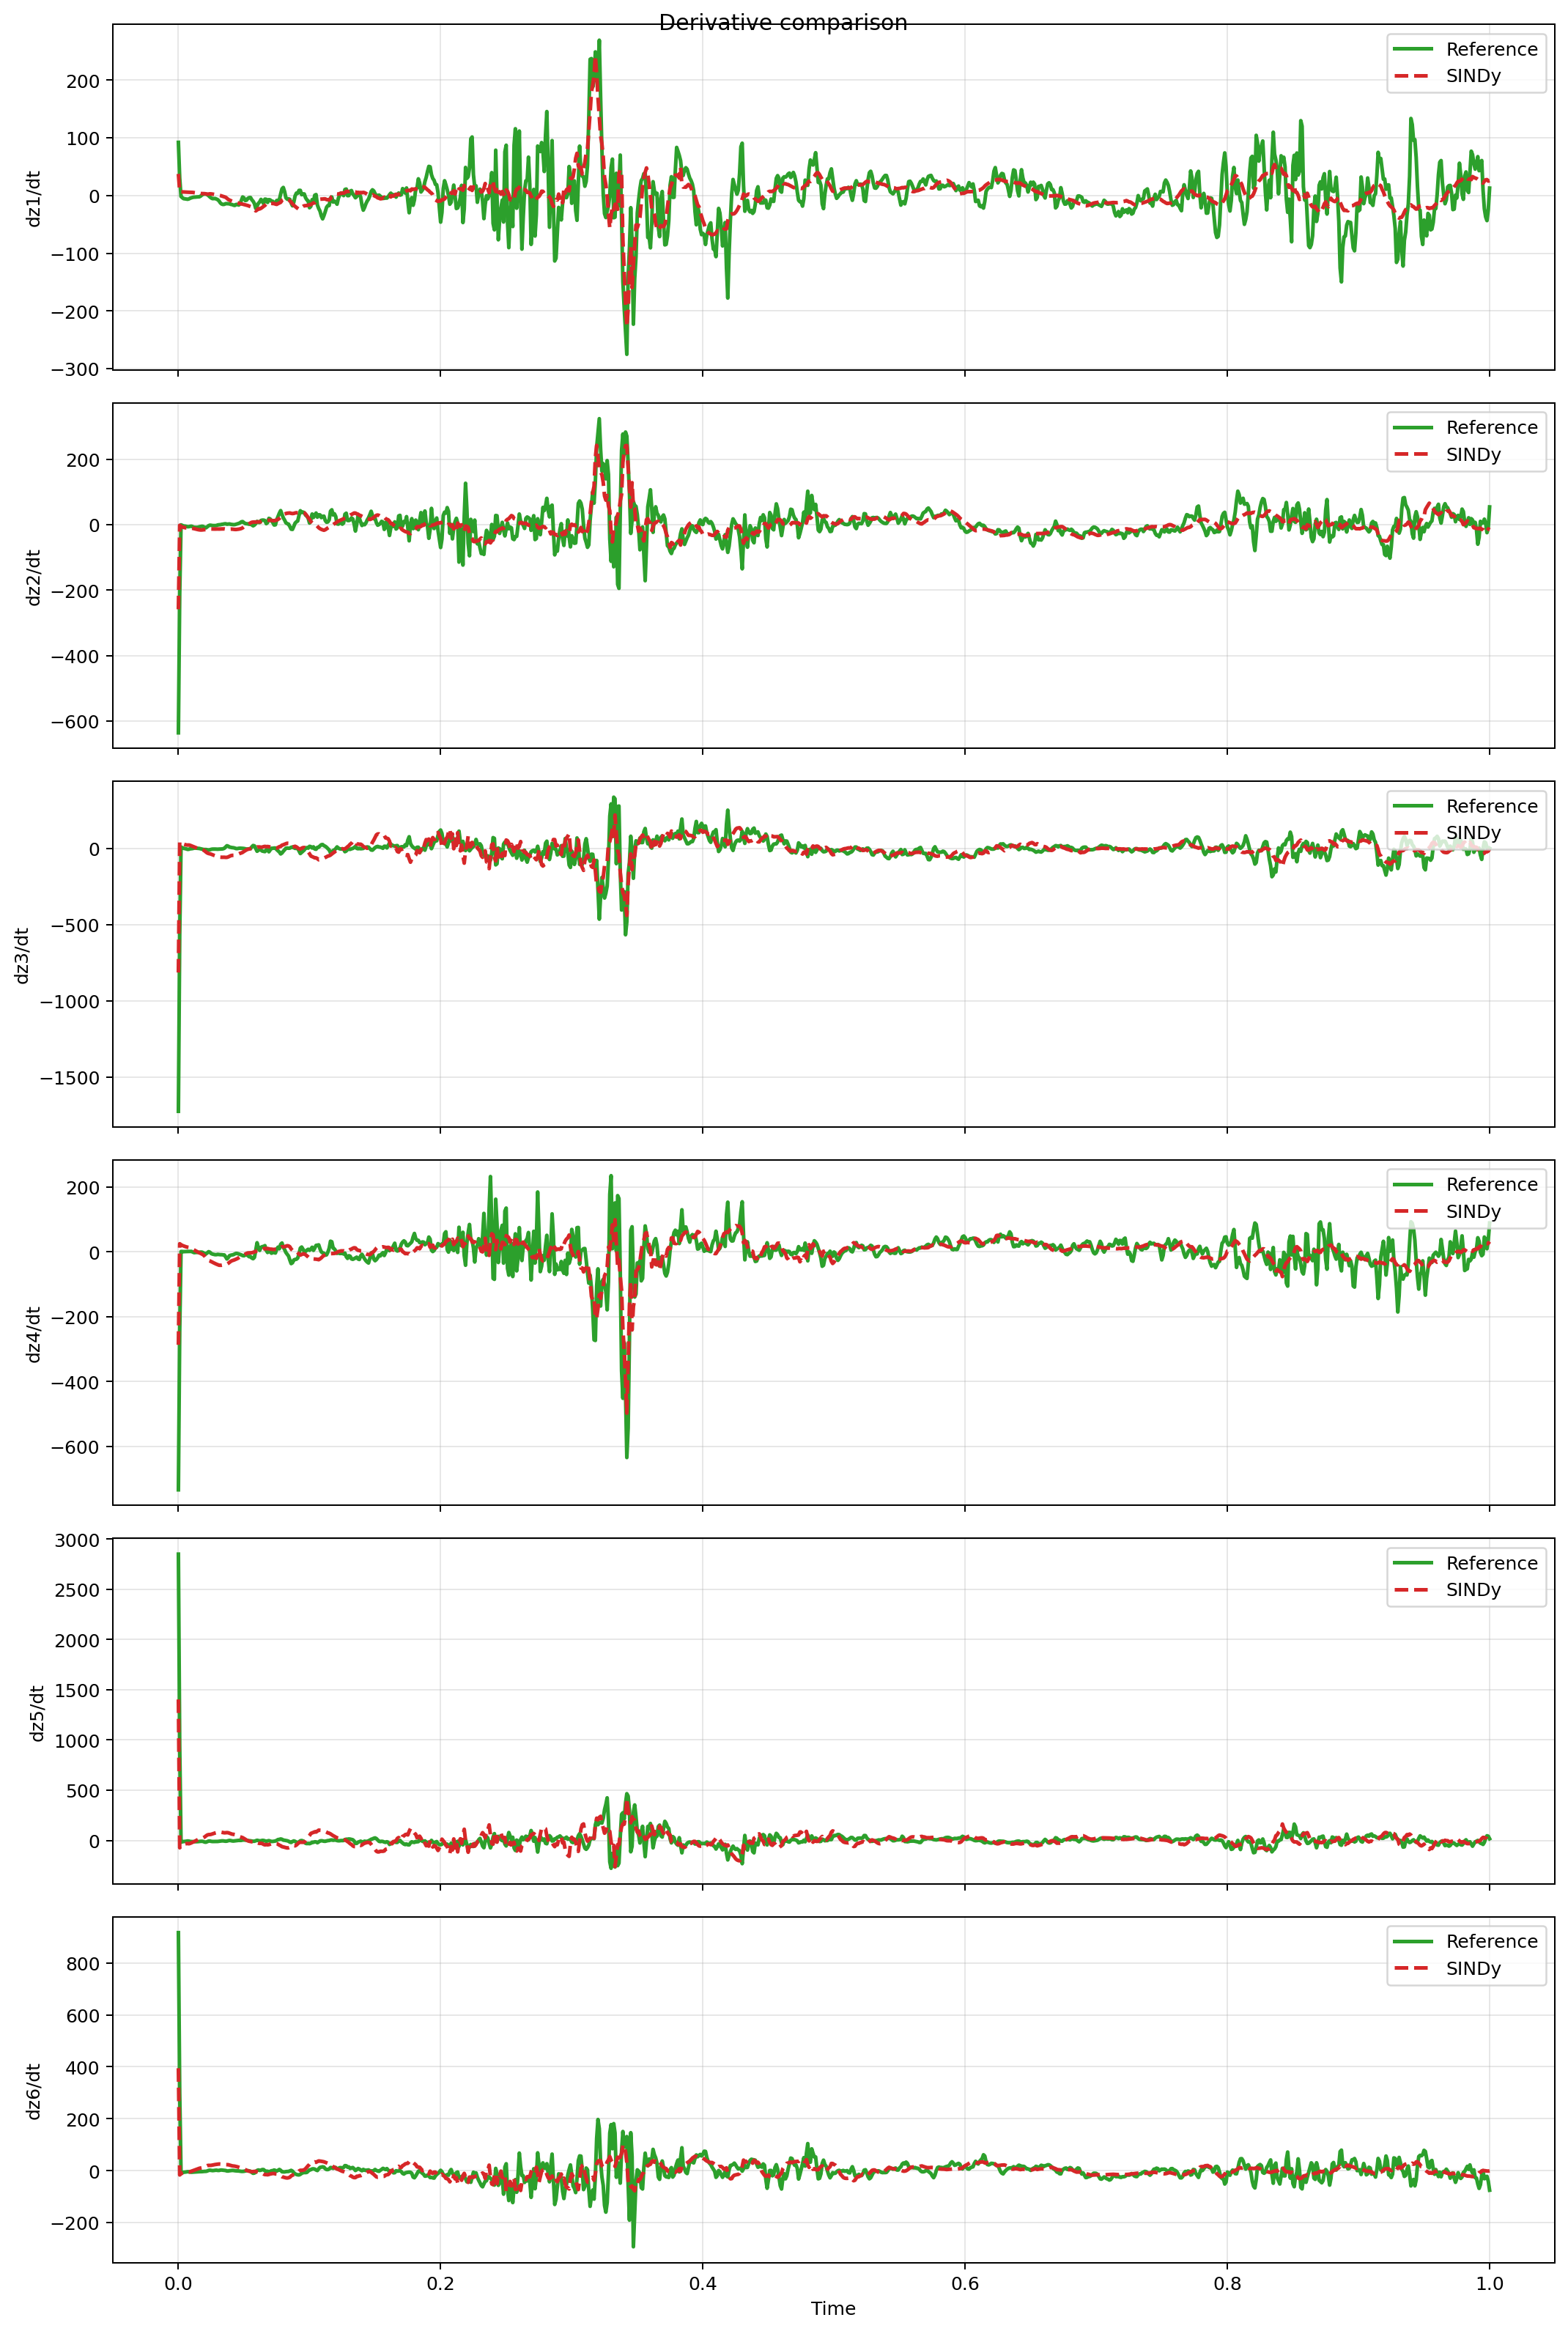
\includegraphics[width=\linewidth]{saes_deriv.png}\caption{Derivadas.}\end{subfigure}
\begin{subfigure}{.49\textwidth}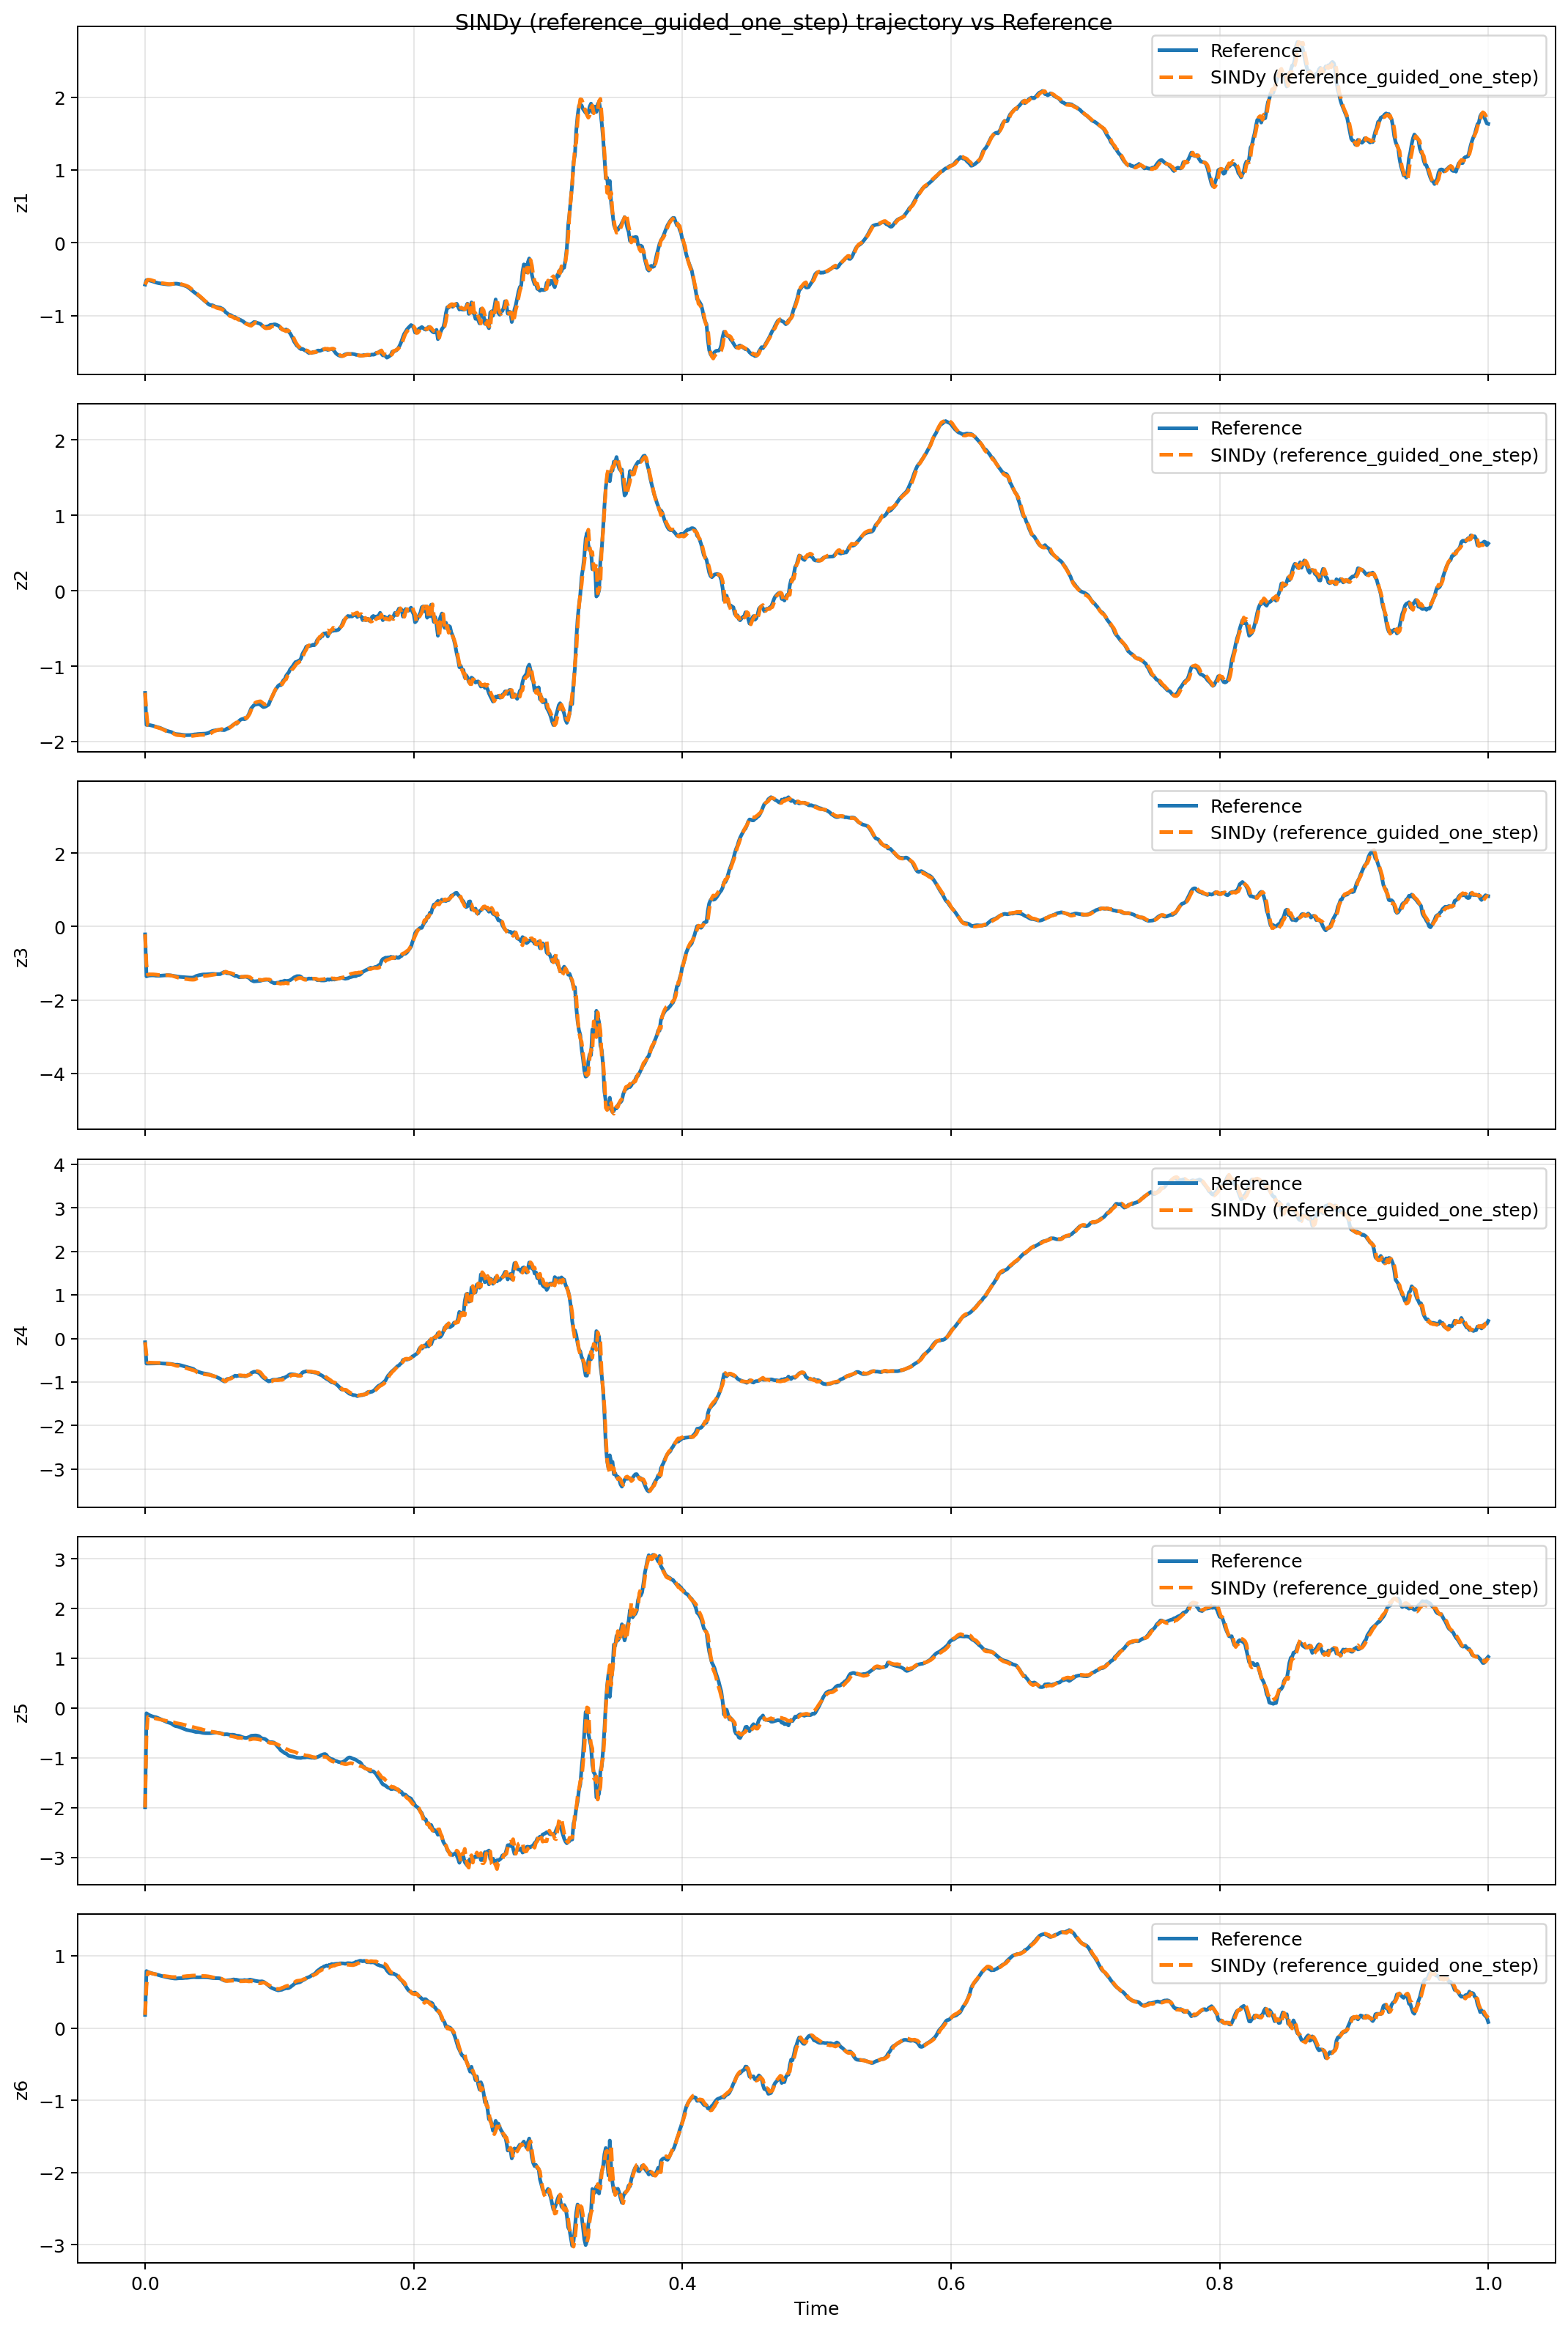
\includegraphics[width=\linewidth]{saes_traj.png}\caption{Trajetória guiada.}\end{subfigure}
\caption{SAE--SINDy: modelo denso e integração livre malsucedida.}\end{figure}

\subsection{SAE--POD--SINDy: estabilização por POD}
Os oito latentes são normalizados e reduzidos a quatro coordenadas POD, preservando 90,95\% da energia. Entre 48 candidatos, 28 atenderam aos limites definidos. O selecionado usa ordem 1, Adalasso, $\alpha=10^{-3}$, Savitzky--Golay 21, termos polinomiais em tempo, sem senos e RK45. A biblioteca tem oito termos por equação e todos os 32 coeficientes são não nulos, portanto não há esparsidade efetiva.

\begin{table}[H]\centering\caption{Métricas SAE--POD--SINDy.}\label{tab:hyb}
\begin{tabular}{lr}\toprule Métrica&Valor\\\midrule
Energia POD latente&0,9095\\Erro de derivada / $R^2$&0,9120 / 0,1682\\Erro de um passo / $R^2$&0,04782 / 0,99771\\Integração livre&bem-sucedida\\Erro livre / $R^2$&0,63368 / 0,59844\\\bottomrule\end{tabular}\end{table}
\lstinputlisting[style=sindyeq,caption={Equações completas SAE--POD--SINDy.}]{equacoes_sae_pod_sindy.txt}
\begin{figure}[H]\centering
\begin{subfigure}{.49\textwidth}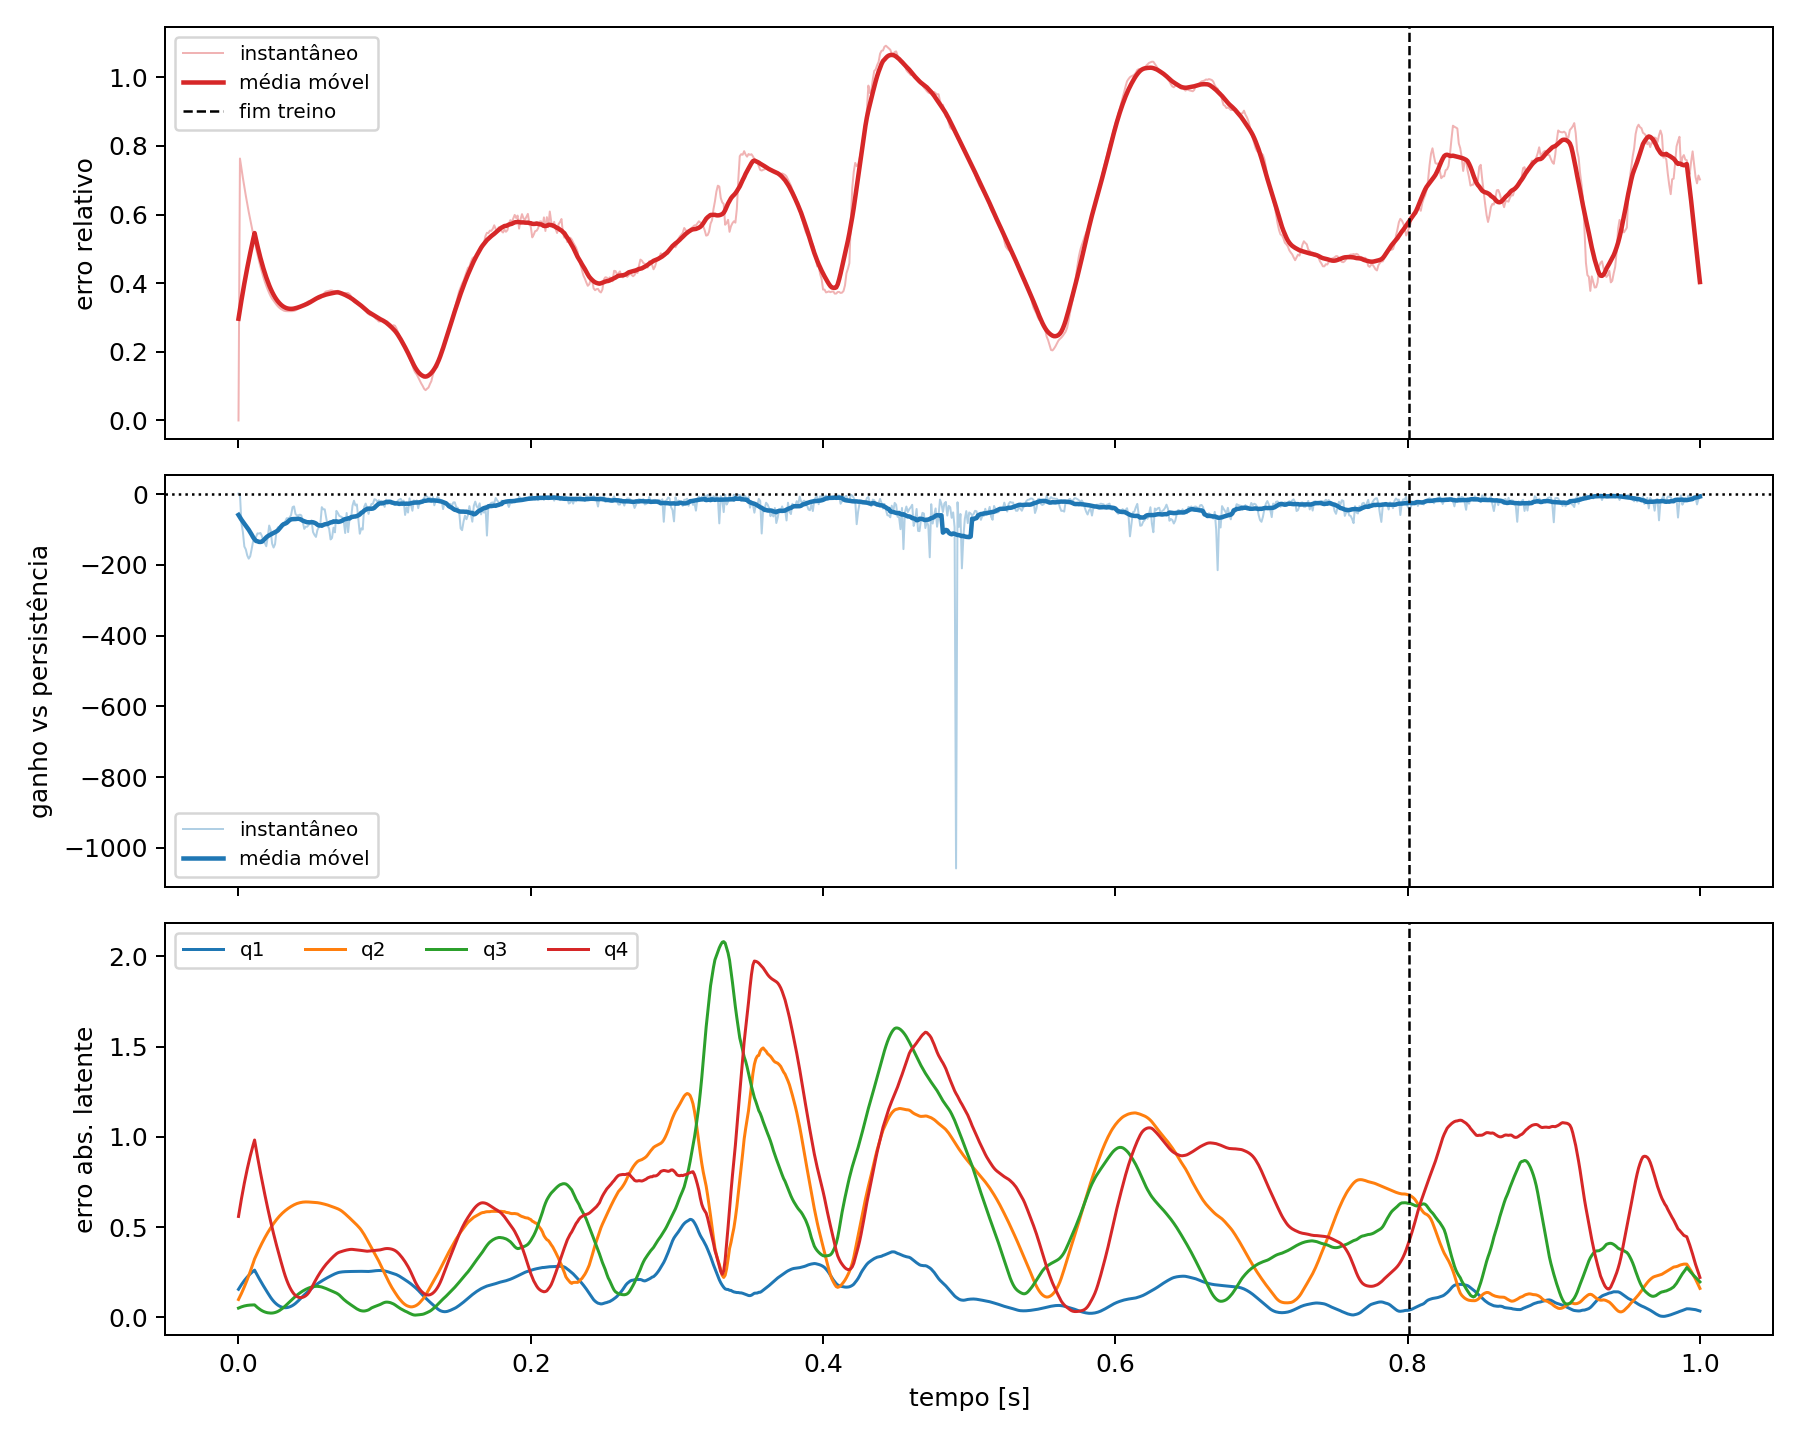
\includegraphics[width=\linewidth]{hyb_curves.png}\caption{Erro temporal.}\end{subfigure}
\begin{subfigure}{.49\textwidth}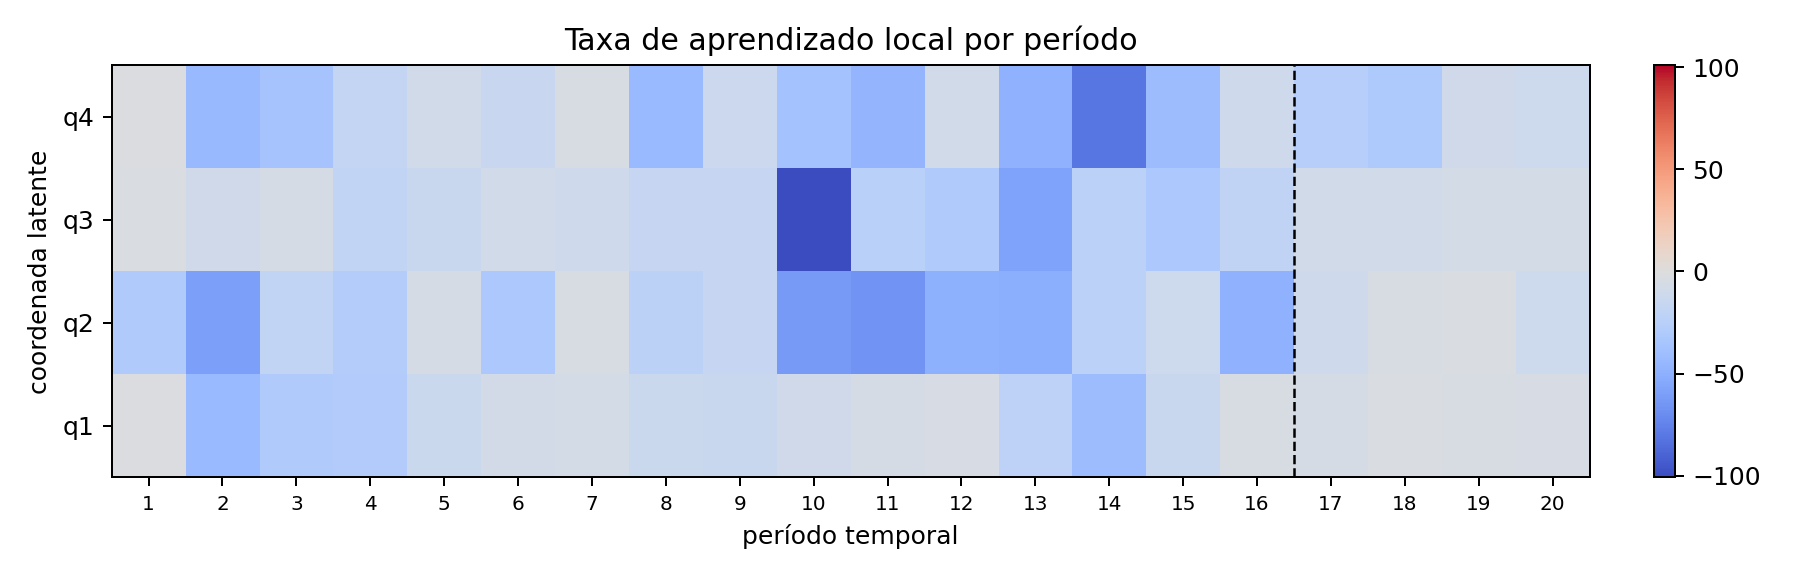
\includegraphics[width=\linewidth]{hyb_map.png}\caption{Mapa das coordenadas.}\end{subfigure}
\caption{Diagnóstico do modelo estabilizado.}\end{figure}
\begin{figure}[H]\centering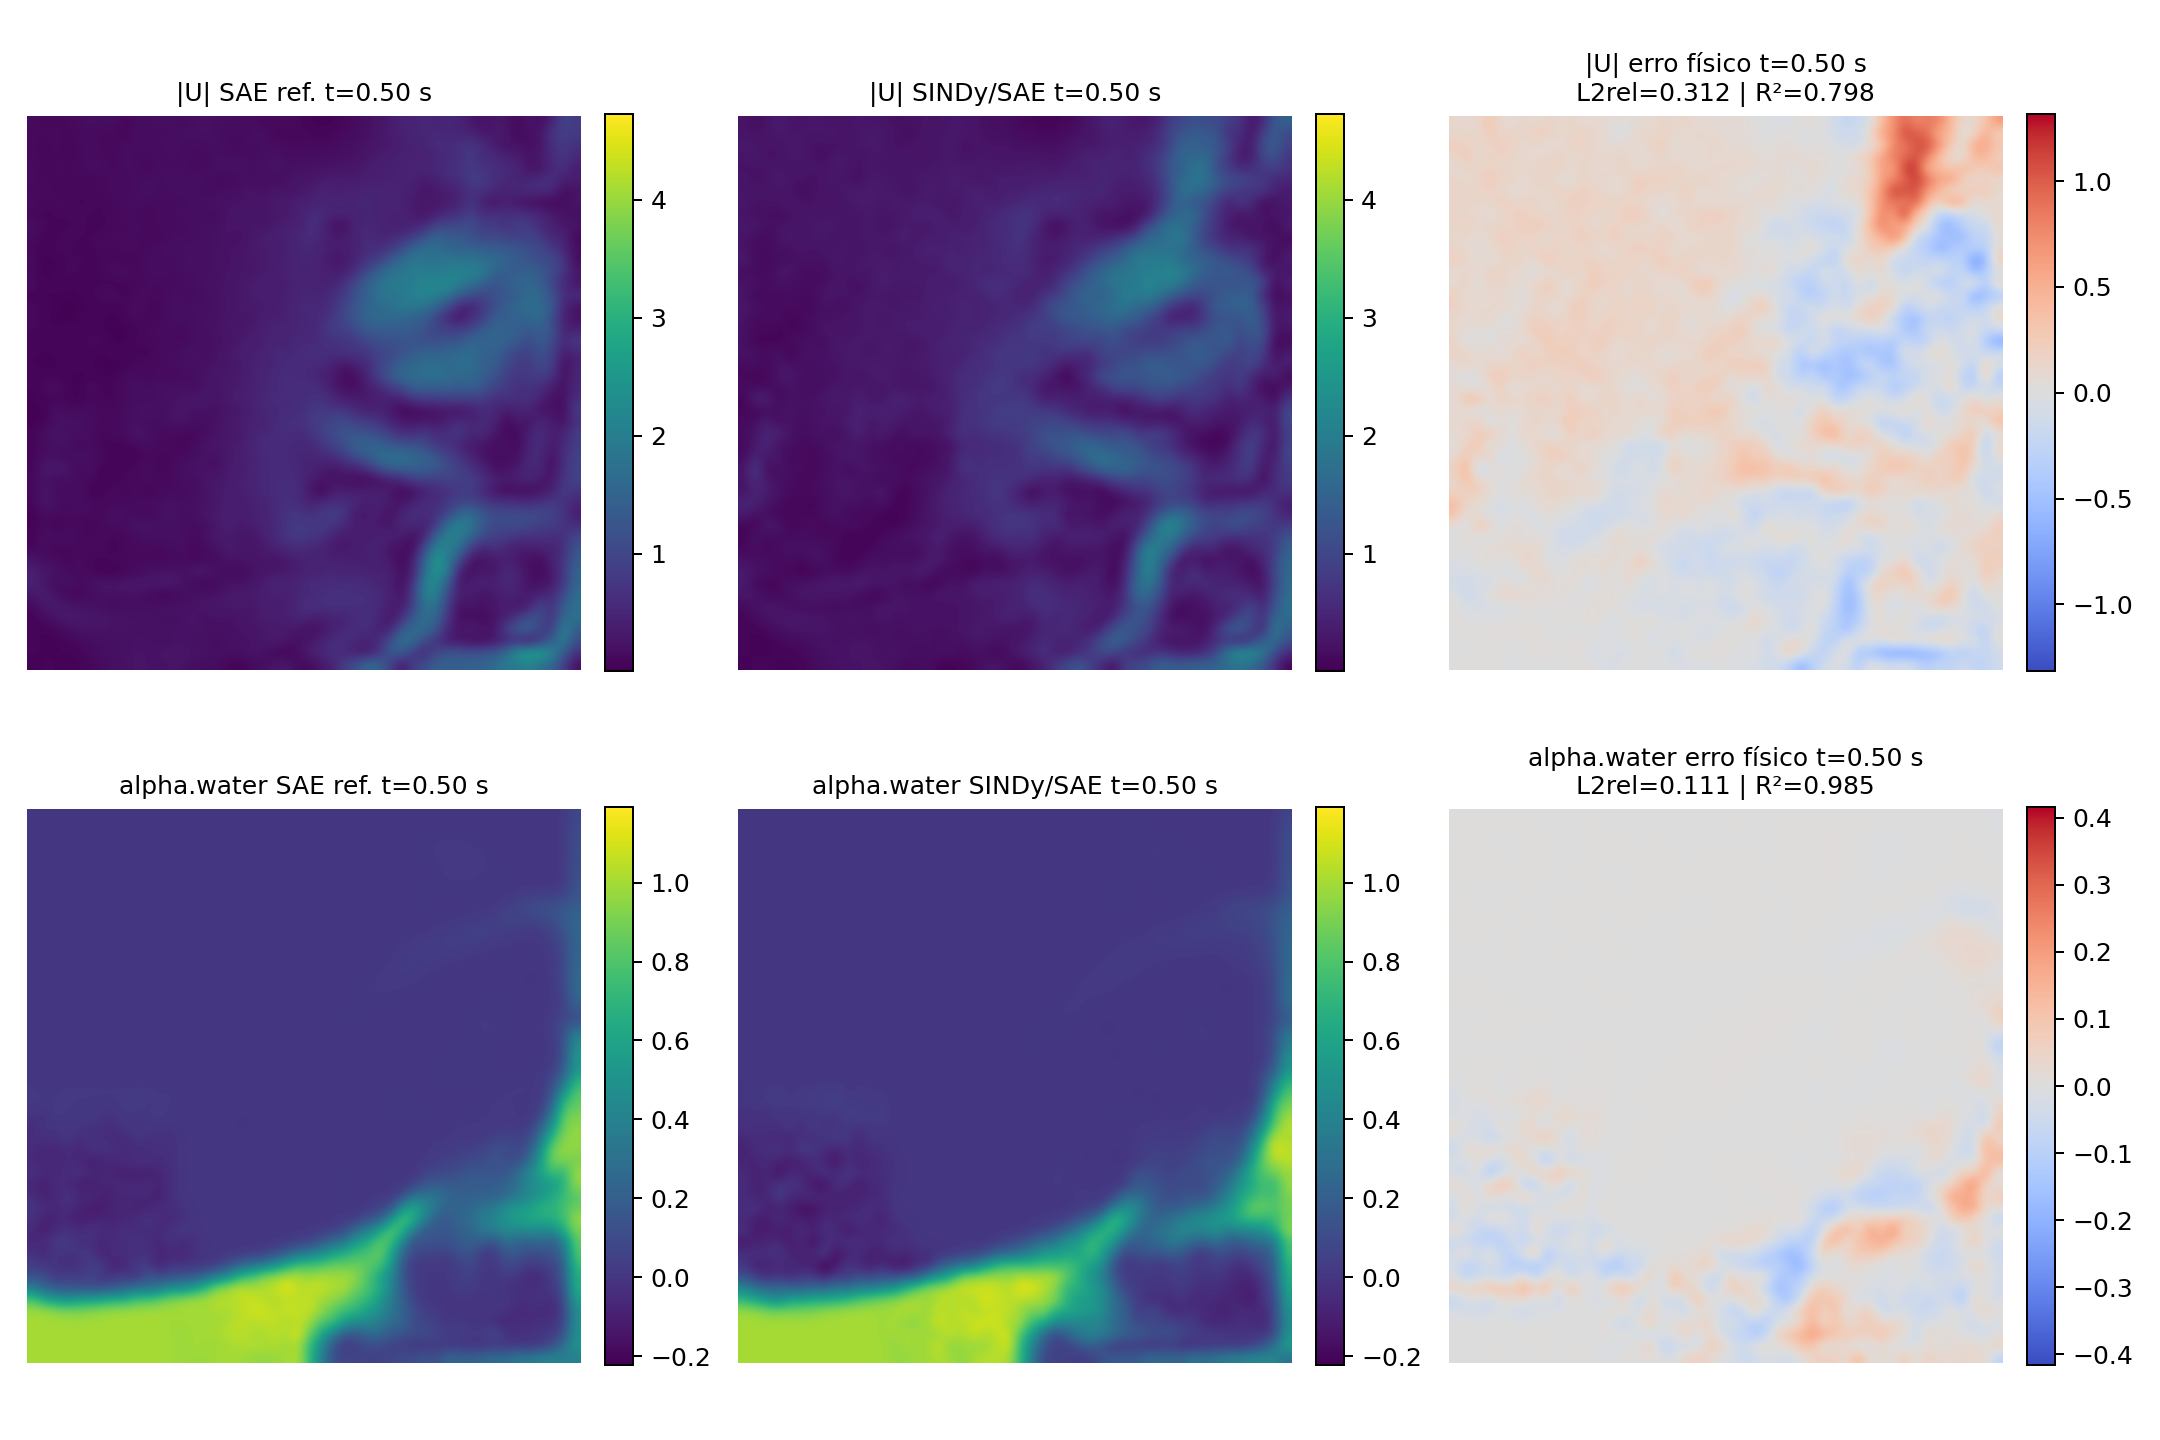
\includegraphics[width=.91\textwidth]{hyb_t05.png}\caption{Campos da integração livre em $t=\SI{0.5}{s}$.}\end{figure}
\begin{figure}[H]\centering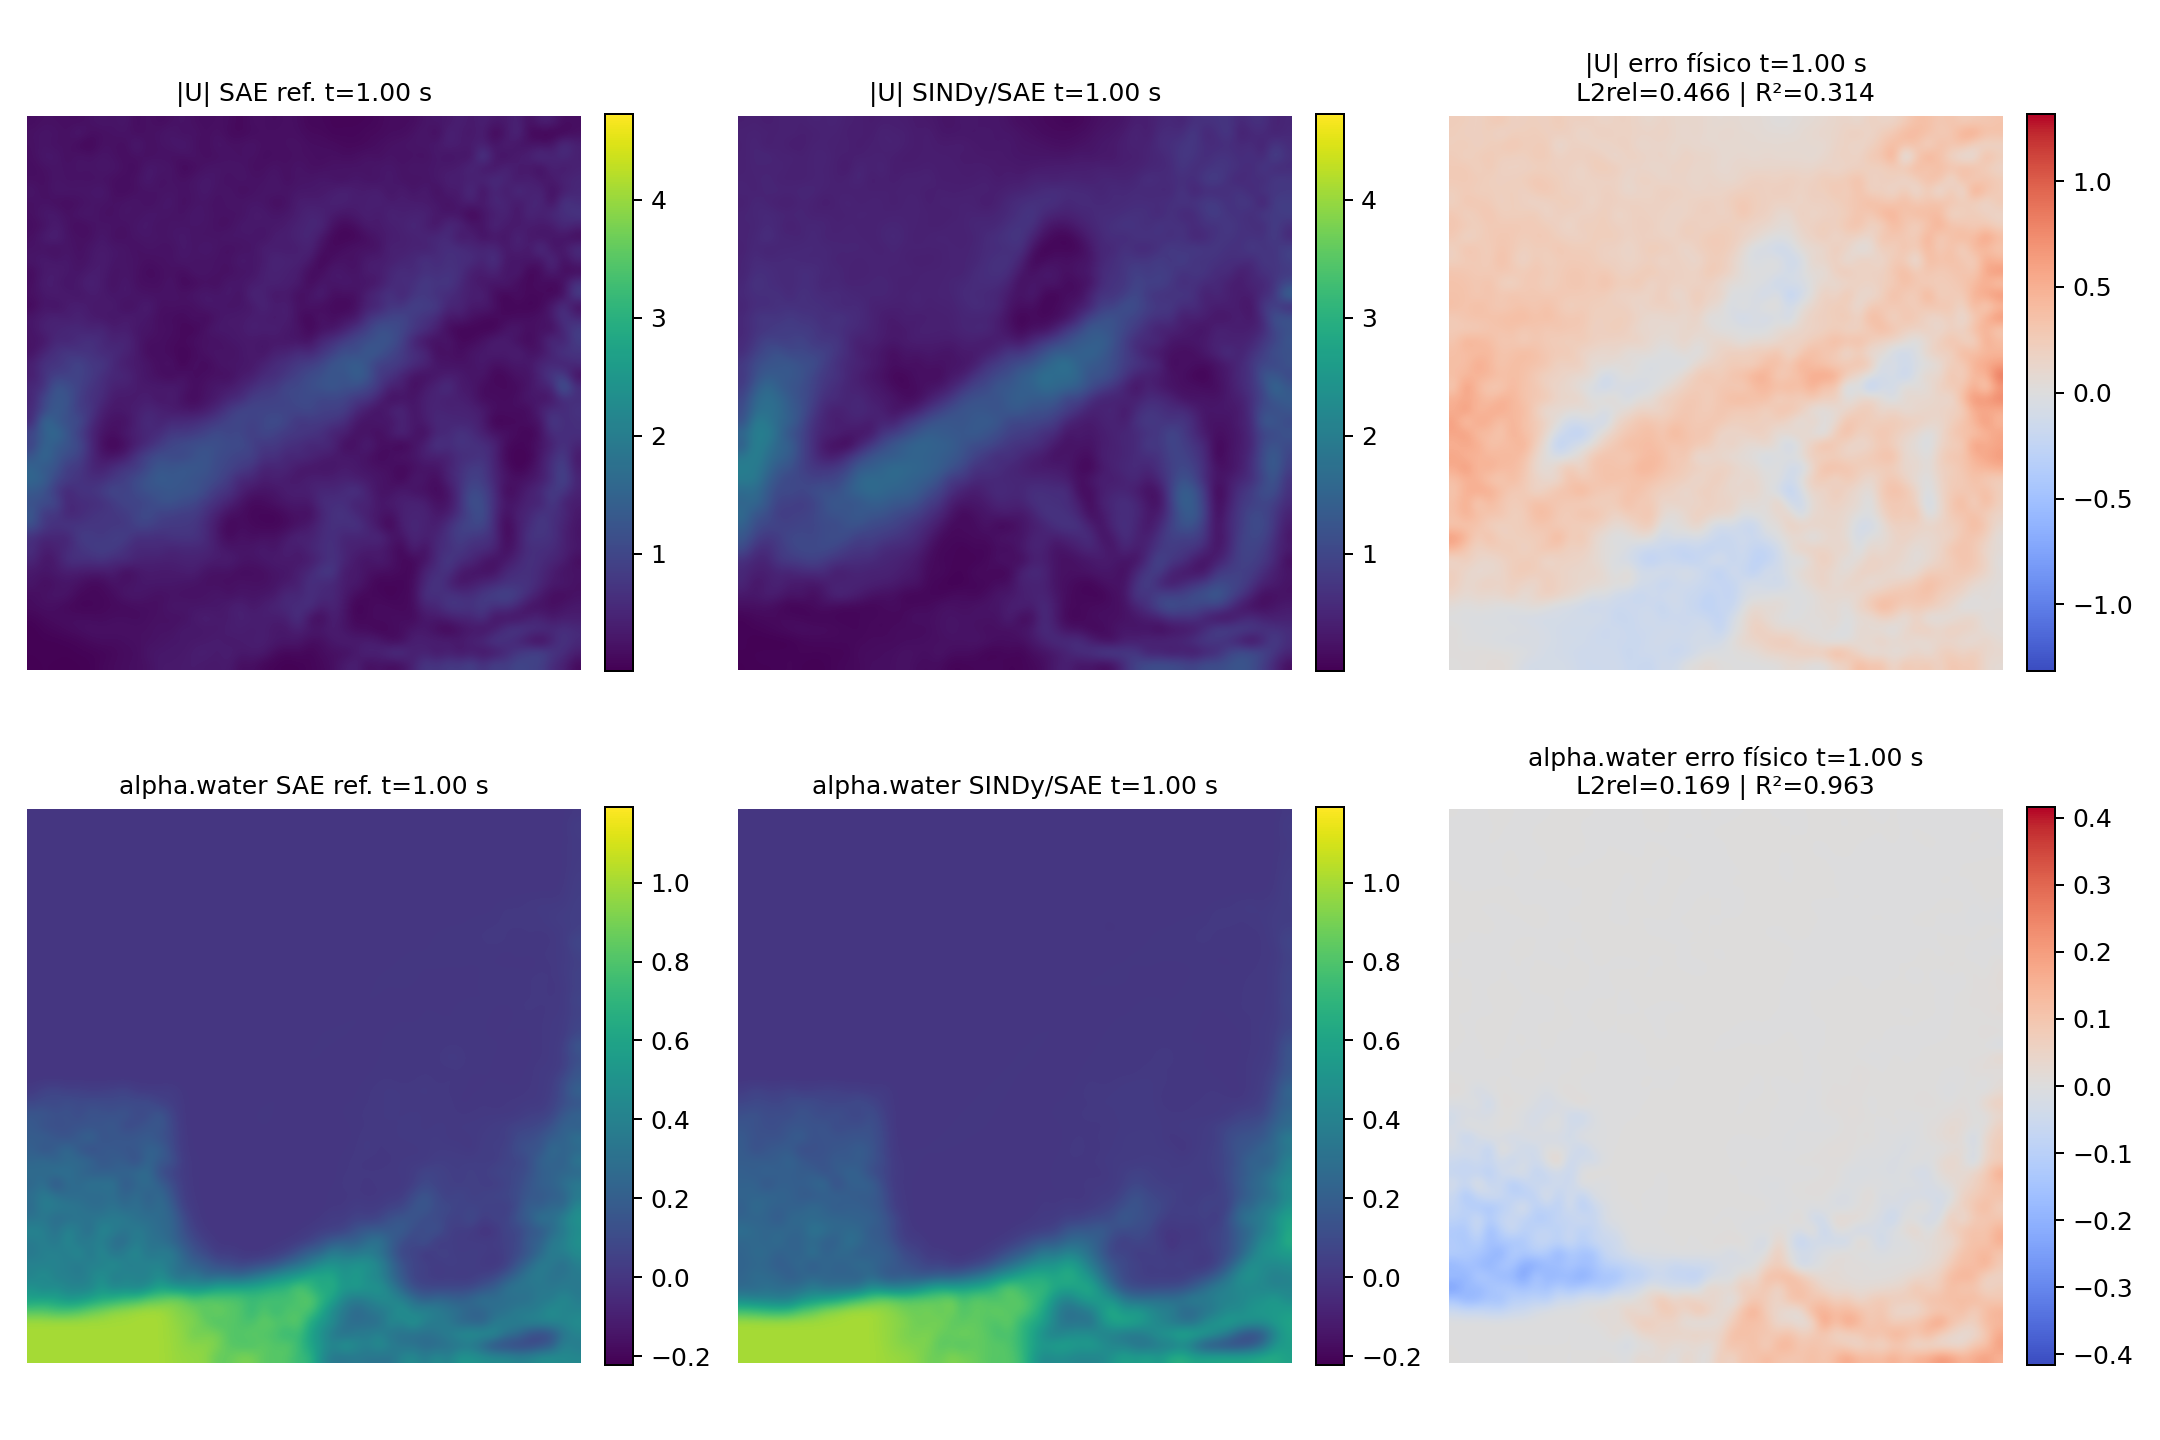
\includegraphics[width=.91\textwidth]{hyb_t10.png}\caption{Campos em $t=\SI{1}{s}$.}\end{figure}

Nos tempos $0;0,25;0,50;0,75;1\,\si{s}$, o erro de $|U|$ é 0,387; 0,268; 0,312; 0,158; 0,466. Para $\alpha_{water}$ é 0,172; 0,241; 0,111; 0,116; 0,169. A interface é mais robusta que a velocidade.

\section{Relação com a POD estabilizadora de Lin, Xiao e Fang}
Lin, Xiao e Fang~\cite{lin2024} propõem SAE--POD--SINDy: o SAE obtém uma variedade não linear, a POD centraliza/ortogonaliza e suaviza seus códigos, e o SINDy descobre a lei temporal. A motivação é que a aleatoriedade do SAE pode produzir coordenadas difíceis para regressão polinomial. Nos exemplos do artigo, a POD melhora correlação e RMSE e pode produzir equações mais simples.

Neste caso, o SAE--SINDy puro falha na integração, enquanto o SAE--POD--SINDy integra até o final. Isso apoia o efeito estabilizador. Porém, diferentemente da transformação equidimensional enfatizada no artigo, aqui há truncamento de oito para quatro modos e perda de 9,05\% da energia latente. O filtro pode remover ruído, mas também dinâmica. O baixo $R^2$ das derivadas, ausência de esparsidade e erro livre 0,634 mostram estabilização parcial, não descoberta perfeita.

\begin{table}[H]\centering\caption{Representação versus dinâmica.}\label{tab:rep}
\begin{tabularx}{\textwidth}{>{\bfseries}l X X}\toprule Caso&O que faz&Conclusão\\\midrule
POD isolada&reconstrói snapshots em subespaço linear&não possui dinâmica\\
SAE isolado&reconstrói snapshots em variedade não linear&não possui dinâmica\\
POD--SINDy&equações nas amplitudes POD&principal falha; busca livre com erro 0,783\\
SAE--SINDy&equações nos latentes&livre falha; sucesso apenas local\\
SAE--POD--SINDy&equações após filtro/rotação POD&livre funciona; erro 0,634\\
\bottomrule\end{tabularx}\end{table}

Assim, não é correto dizer que todo caso isolado com SINDy apenas representa dados: ele tenta modelar dinâmica. Contudo, como suas integrações livres falham ou têm erro alto, a evidência obtida é predominantemente local. A POD estabilizadora não cria a dinâmica; ela fornece coordenadas mais condicionadas para o SINDy.

\section{Pontos positivos, negativos e recomendações}
\subsection*{Positivos}
\begin{itemize}
\item 10001 snapshots e passo pequeno;
\item POD com 99,62\% da energia e erro 6,17\% em 50 modos;
\item equações completas e diagnósticos temporais salvos;
\item POD latente torna possível a integração livre;
\item campos decodificados de $\alpha$ mantêm $R^2$ alto nos tempos avaliados.
\end{itemize}
\subsection*{Negativos}
\begin{itemize}
\item POD inclui $k$ inexistente como zero; SAE usa $\rho$, impedindo comparação direta;
\item SAE generaliza mal no split temporal;
\item POD--SINDy principal e SAE--SINDy falham em integração livre;
\item modelo híbrido retém todos os termos, tem erro de derivada 0,912 e erro livre 0,634;
\item dependência explícita de $t$ reduz generalidade;
\item Euler de primeira ordem, malha quase 2D e ausência de verificação/validação.
\end{itemize}
\subsection*{Recomendações}
\begin{enumerate}
\item Unificar canais POD e SAE, removendo $k$ e evitando redundância $\rho$--$\alpha$.
\item Fazer o leitor falhar quando um campo obrigatório estiver ausente.
\item Melhorar o SAE com mais amostras, maior taxa inicial e penalização temporal/dinâmica.
\item Comparar POD latente equidimensional com POD truncada, registrando energia, suavidade e erro livre.
\item Selecionar SINDy pela integração livre em validação temporal; normalizar biblioteca e testar STLSQ/SR3/Adalasso.
\item Avaliar massa, limites de $\alpha$, energia cinética e independência de malha/passo.
\end{enumerate}

\section{Conclusão}
A POD fornece a melhor reconstrução estática, enquanto o SAE sofre forte extrapolação temporal. POD e SAE isolados representam snapshots, não dinâmica. Os SINDy puros tentam identificar dinâmica, mas não produzem integração livre confiável. A POD estabilizadora permite integração completa, em concordância qualitativa com Lin, Xiao e Fang, porém com truncamento de energia, sistema não esparso e erro livre 0,634. Portanto, ela melhora a estabilidade, mas o modelo reduzido ainda não está validado para previsão autônoma precisa.

\appendix\section{Arquivos principais}
\small\begin{itemize}
\item OpenFOAM: \path{system/controlDict}, \path{fvSchemes}, \path{fvSolution}, \path{blockMeshDict}, \path{constant/momentumTransport}.
\item POD: \path{POD/resultados/resultados_pod_completos.npz}.
\item SAE: \path{SAE/resultados/sae_dense.keras}, \path{sae_dense_metrics.npz}, \path{latents.npz}.
\item SINDy: JSON, CSV, NPZ e equações em \path{SINDy/resultados}.
\end{itemize}\normalsize
\begin{thebibliography}{9}
\bibitem{sirovich} L. Sirovich. Turbulence and the dynamics of coherent structures. \emph{Quarterly of Applied Mathematics}, 45, 1987.
\bibitem{hinton} G. E. Hinton e R. R. Salakhutdinov. Reducing the dimensionality of data with neural networks. \emph{Science}, 313, 2006.
\bibitem{brunton} S. L. Brunton, J. L. Proctor e J. N. Kutz. Discovering governing equations from data by sparse identification of nonlinear dynamical systems. \emph{PNAS}, 113, 2016.
\bibitem{lin2024} X. Lin, D. Xiao e F. Fang. Data discovery of low dimensional fluid dynamics of turbulent flows. \emph{arXiv:2401.05449}, 2024. \href{https://arxiv.org/abs/2401.05449}{arxiv.org/abs/2401.05449}.
\bibitem{openfoam} OpenFOAM Foundation. \emph{OpenFOAM 13 documentation}.
\end{thebibliography}\end{document}
